\chapter{एमएस एक्सेल का परिचय}

माइक्रोसॉफ्ट (एमएस) एक्सेल एक स्प्रेडशीट एप्लीकेशन हैं, जिसे माइक्रोसॉफ्ट द्वारा विकसित किया गया हैं। एक्सेल सबसे ज्यादा इस्तेमाल की जाने वाली स्प्रेडशीट एप्लीकेशन में से एक है और यह माइक्रोसॉफ्ट ऑफिस सुइट का हिस्सा है। एक स्प्रेडशीट मूलतः रो और कॉलमो की एक मैट्रिक्स होती हैं। डाटा को प्रविष्ट (एंटर) करने, संपादित (एडिट) करने, विश्लेषित (अनलाइज) करने और संग्रहित (स्टोर) करने में स्प्रैडशीट बहुत उपयोगी होती है। एक्सेल का उपयोग करके संख्यात्मक डाटा के साथ अंकगणितीय कार्य जैसे कि जोड़ना, घटाना, गुणा करना और भाग देना आदि किया जा सकता है। इसके अलावा आप नंबर को व्यवस्थित (सॅार्ट) कर सकते हैं और साधारण वित्तीय, अंकगणितीय और सांख्यिकीय आँकड़ों से संबंध्तिद्ध सूत्रों (फार्मुलो) का उपयोग कर सकते हैं। संख्याओं को ग्राफिकली प्रदर्शित करने के लिए भी, आप एक्सेल का उपयोग कर, एक चार्ट बना सकते हैं। इस पुस्तक में एक्सेल, पावर पॉइंट, और पिक्चर मेनेजर की व्याख्या करने के लिए, एमएस ऑफिससुइट 2007 संस्करण का उपयोग किया गया हैं और सभी दिए गए चित्र (पिक्चर) और उदाहरण तदनुसार हैं।

\paragraphTitle{एक्सेल प्रारंभ करना}
आप एक्सेल को उसी तरह से प्रारंभ कर सकते है जैसे आप माइक्रोसॉफ्ट ऑफिस सुइट में हर एप्लीकेशन को प्रारंभ करते हैं, जैसे कि वर्ड, पावर पॉइंट, एक्सेस आदि। एक्सेल को स्टार्ट मेनू से निम्न प्रकार से प्रारंभ कर सकते हैंः

\begin{descriptionSimple}{चरण 4:}
\item[चरण 1] स्क्रीन के निचले-बाएँ कोने में टास्क बार पर \textbf{स्टार्ट} बटन क्लिक करें
\item[चरण 2] मेनू से \textbf{आल प्रोग्राम} विकल्प पर क्लिक करें
\item[चरण 3] प्रोग्राम्स की सूची से \textbf{माइक्रोसॉफ्ट ऑफिस} का चयन करें
\item[चरण 4] \textbf{माइक्रोसॉफ्ट ऑफिस एक्सेल 2007} पर क्लिक करें
\end{descriptionSimple}
\newpage

\begin{figure}[H]
\centering
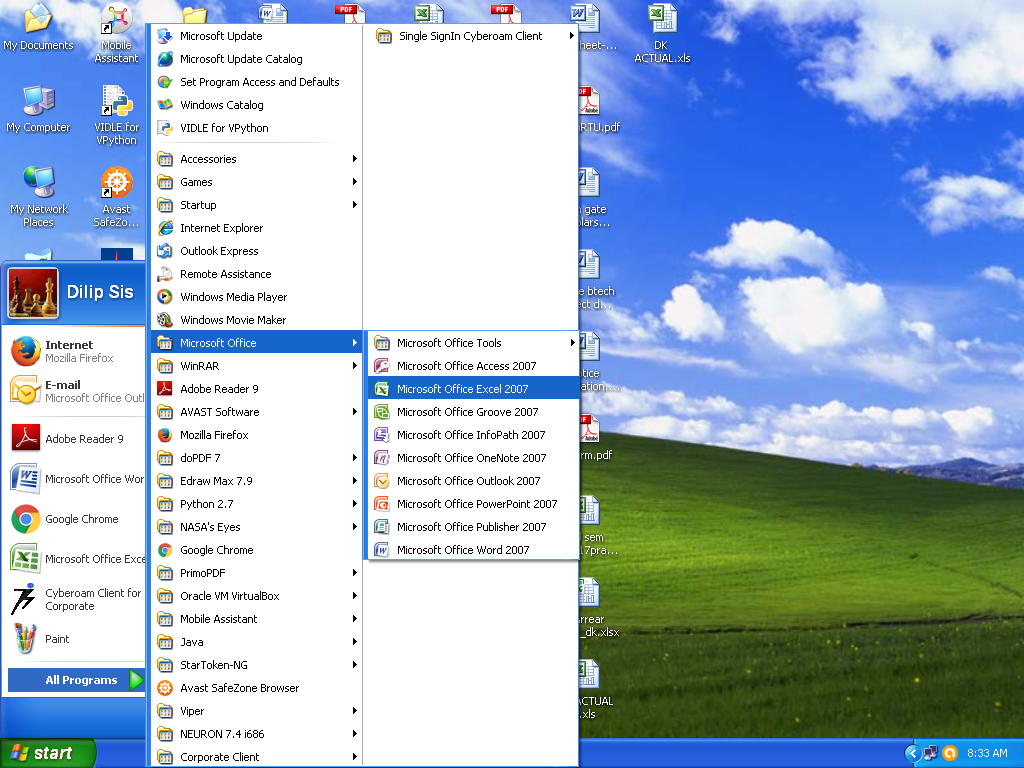
\includegraphics[scale=0.3]{src/images/chapter1_fig01.png}
\caption{एमएस एक्सेल 2007 एप्लीकेशन लॉन्च हो जाएगी और निम्न एमएस एक्सेल 2007 विंडो खुलेगी।}\label{chap1_fig1}
\end{figure}

\begin{figure}[H]
\centering
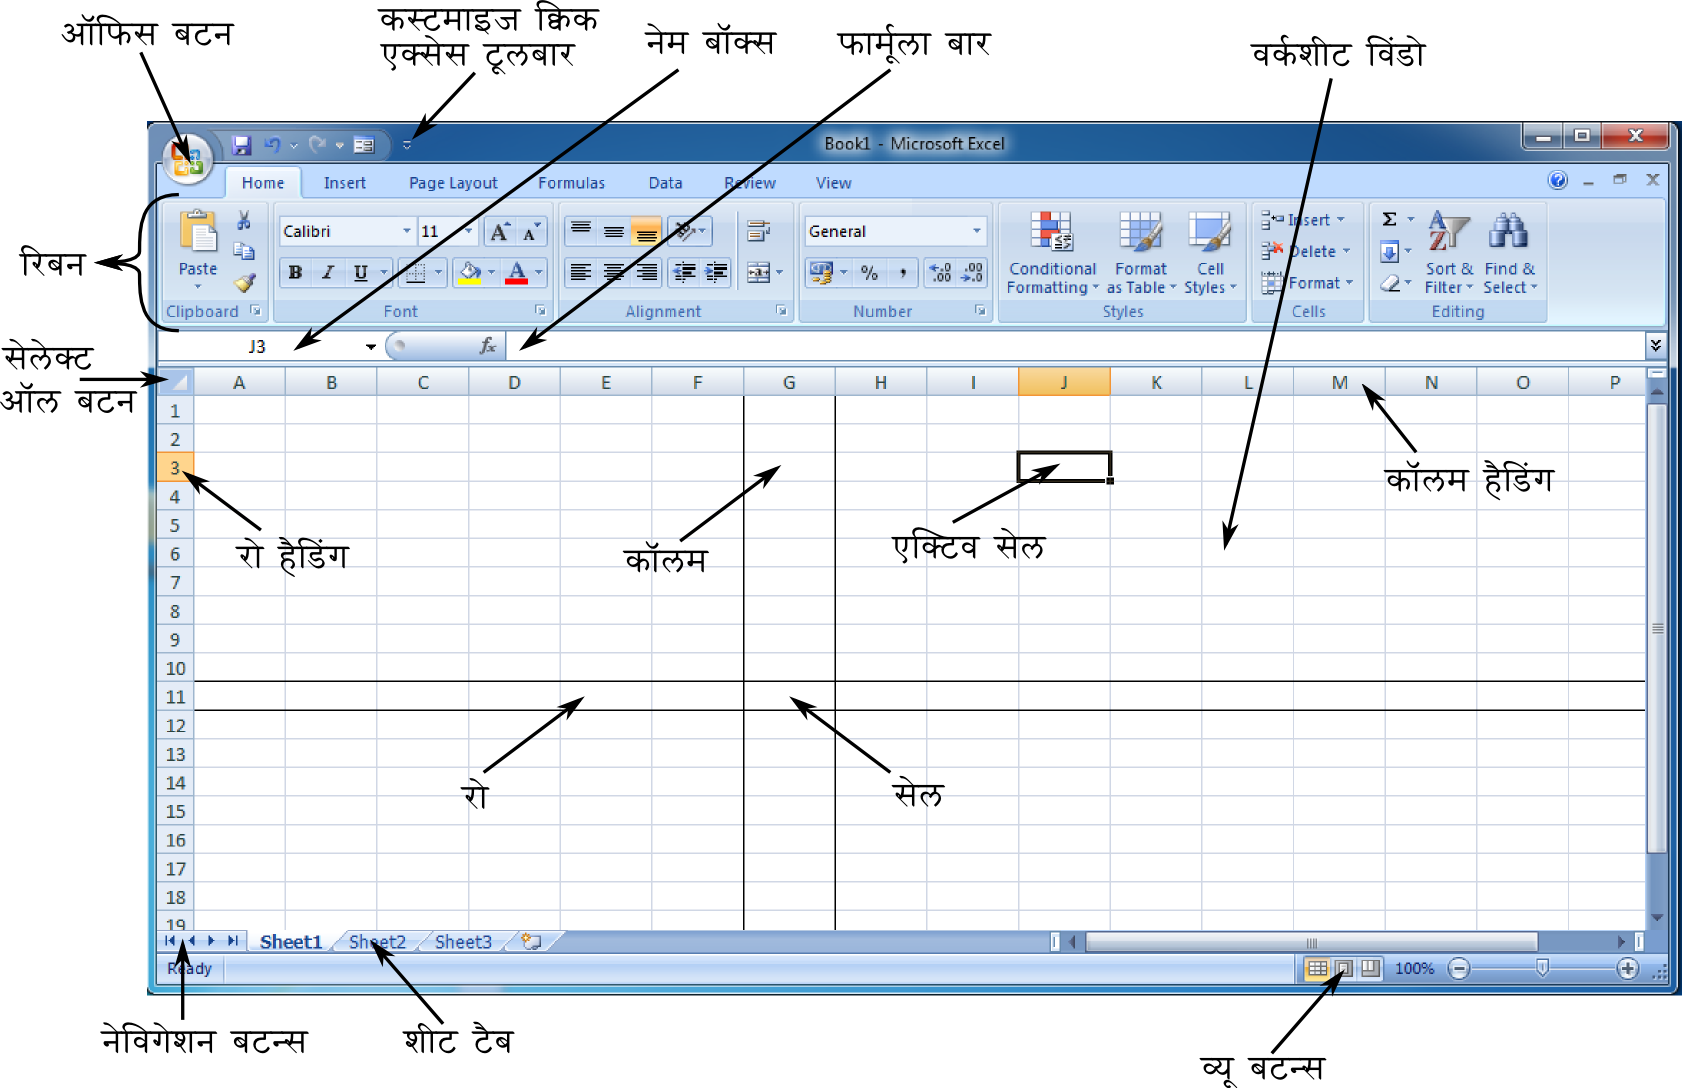
\includegraphics[scale=0.32]{src/images/chapter1_fig02.png}
\end{figure}

\section{एमएस वर्ड और एमएस एक्सेल के मध्य तुलना}\label{id-1.1}

माइक्रोसॉफ्ट एक्सेल और माइक्रोसॉफ्ट वर्ड, माइक्रोसॉफ्ट ऑफिस सुइट में दो एप्लीकेशन सॉफ्टवेयर प्रोग्राम हैं। हालांकि वे एक साथ काम करने के लिए बने हैं, पर उनमे अपनी अलग-अलग खुबिया/स्ट्रेंन्थस् हैं। एक्सेल प्राथमिक रूप से संख्यात्मक परिकलन के लिए है, जबकि वर्ड सबसे पहले एक शब्द संसाधक (प्रोसेसर) होता हैं। एक्सेल एक स्प्रेडशीट प्रोग्राम है जो कि रिकॉर्ड और सांख्यिक डेटा का विश्लेषण करने के लिए उपयोग मे लिया जाता हैं। दूसरे हाथ पर, वर्ड एक शब्द संसाधक एप्लीकेशन हैं, जिसे दस्तावेज जैसे पत्र या निबंध लिखने के लिए उपयोग किया जाता हैं, जहाँ आसानी से पढ़े जा सकने वाले एक प्रिंट करने योग्य दस्तावेज प्रदान करने के लिए, टेक्स्ट स्वरूपण बहुत आवश्यक होता हैं।

आप किसी वर्ड दस्तावेज में टेबल सम्मिलित कर सकते हैं या एक एक्सेल सेल के अंदर पूरे पैराग्राफ को लिख सकते हैं, और दोनों ही एप्लीकेशन प्रिंट करने योग्य दस्तावेज बना सकते हैं। इसलिए, एक का उपयोग कुछ हद तक दूसरे के फंक्शन अनुकरण (सिमुलेट) करने के लिए किया जाना संभव हैं।

लेकिन प्रत्येक एप्लीकेशन मे अपनी कुछ विशेषता होती है जो उन्हे अपने कार्य को अच्छी तरह सेे करने के लिए अनुकूल बनाती है। वर्ड के फॉन्ट, अनुच्छेद, और पेज स्वरूपण (फॉर्मेटिंग) विकल्प दस्तावेज बनाने को आसान कर देते है, जोकि एक्सेल में काफी मुश्किल हैं। जबकि एक्सेल में विश्लेषण, सूत्रों (फॉर्मुलास) और सशर्त कथन (कंडीशनल स्टेटमेंट्स) की गणना करने की क्षमता होती हैं। जैसे इससे सभी प्रवेश किये गये डेटा का योग (सम) और उनके औसत लेना एवं और भी अधिक जटिल समीकरणों को सरलता से हल किया जा सकता है। आपको इस प्रकार की क्षमता वर्ड के भीतर नहीं मिलेगी।

\begin{table}[h]
\centering
\caption{एमएस वर्ड और एमएस एक्सेल के मध्य तुलना}
\begin{tabular}{@{}|l|p{6cm}|p{6cm}@{}|}
\hline
\multicolumn{1}{|c}{\textbf{क्र.सं.}} & \multicolumn{1}{|c|}{\textbf{एमएस वर्ड}} & \multicolumn{1}{c|}{\textbf{एमएस एक्सेल}} \\
\hline
1 & शब्द संसाधक (प्रोसेसर) एप्लीकेशन & स्प्रेडशीट एप्लीकेशन \\
\hline
2 & पत्र, निबंध लेखन के लिए उपयोगी & सारणीबद्ध दस्तावेज बनाने के लिए उपयोगी \\
\hline
3 & जहाँ टेक्स्ट स्वरूपण (फॅार्मेटिग) आवश्यक है, वहॉ इसका उपयोग किया जाता हैं & रिकॉर्ड और सांख्यिक डेटा का विश्लेषण करने के लिए इसका उपयोग किया जाता हैं \\
\hline
4 & एक्सल तालिकाओं को एक वर्ड दस्तावेज के अंदर सम्मिलित किया जा सकता हैं & वर्ड दस्तावेज को किसी एक्सल तालिका के अंदर सम्मिलित नहीं किया जा सकता हैं \\
\hline
5 & उन्नत स्वरूपण (फॅार्मेटिग) सुविधाए होती हैं & उन्नत स्वरूपण (फॅार्मेटिग) सुविधाए नहीं होती हैं \\
\hline
6 & कस्टम समीकरण और सूत्र नही लिखे जा सकते & कस्टम समीकरण और सूत्र लिखे जा सकते \\
\hline
\end{tabular}
\end{table}


\section{वर्कशीट और वर्कबुक}\label{id-1.2}

जब आप एक्सेल प्रारंभ करते हैं, स्वचालित रूप से एक नई, रिक्त वर्कबुक शुरू हो जाती हैं। एक साधारण एक्सेल फाइल को वर्कबुक कहा जाता हैं, जोकि अलग अलग चीजें जैसे वर्कशीट, चार्ट शीट और कई छोटे प्रोग्राम शामिल कर सकती हैं। प्रत्येक वर्कबुक मे एक या एक से अधिक वर्कशीटे हो सकती हैं। एक एक्सेल वर्कशीट एकल (सिंगल) स्प्रेडशीट हैं, जो रो (संख्याओं द्वारा निर्दिष्ट) और कॉलमों (अक्षरों द्वारा निर्दिष्ट) की मैट्रिक्स होती है। कॉलम और रो के मिलान (इंटरसेक्शन) को सेल कहते हैं। स्प्रैडशीट में प्रत्येक सेल का एक सेल ऐड्रेस होता है जो कॉलम अक्षर और रो संख्या से मिलकर बनता है। सेल में टेक्स्ट, संख्याएँ, गणितीय फॉर्मूले हो सकते हैं। एक सेल, उसी वर्कशीट, एक ही वर्कबुक या किसी अन्य वर्कबुक में किसी अन्य सेल को संदर्भित (रफरेन्स) कर सकता हैं। स्टेटस बार के ठीक ऊपर स्थित वर्कशीट टैब दबाकर वर्कबुक में वर्कशीटों पर पहुँच प्राप्त की जा सकती है। डिफॉल्ट रूप से एक्सेल, प्रत्येक वर्कबुक में तीन वर्कशीट {\rm Sheet1, Sheet2,} और {\rm Sheet3} नाम के साथ प्रदान करता हैं। आवश्यकता के अनुसार आप, एक वर्कबुक में अतिरिक्त वर्कशीट जोड़ सकते हैं, और उन्हे हटा सकते हैं। आप एक नई वर्कबुक में डिफॉल्ट रूप से दिखाई देने वाले वर्कशीटो की संख्या को भी बदल सकते~हैं। 

\section{वर्कबुक बनाना}\label{id-1.3}

यदि आप एमएस एक्सेल 2007 में काम कर रहे हैं और एक नई एक्सेल फाइल में काम शुरू करना चाहते हैं, तो आप एक नई वर्कबुक निम्न चरणों का पालन करके बना सकते हैंः 
\begin{descriptionSimple}{चरण 1:}
\item[चरण 1] \textbf{ऑफिस बटन} पर क्लिक करें
\item[चरण 2] \textbf{न्यु} का चयन करें
\item[चरण 3] \textbf{ब्लेंक वर्कबुक} चिह्न क्लिक करें
\item[चरण 4] \textbf{क्रिएट} बटन क्लिक करें
\end{descriptionSimple}
\begin{figure}[H]
\centering
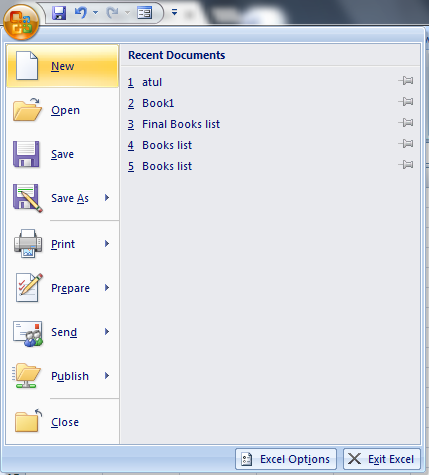
\includegraphics[scale=0.4]{src/images/chapter1_fig03.png}
\end{figure}
\begin{figure}[H]
\centering
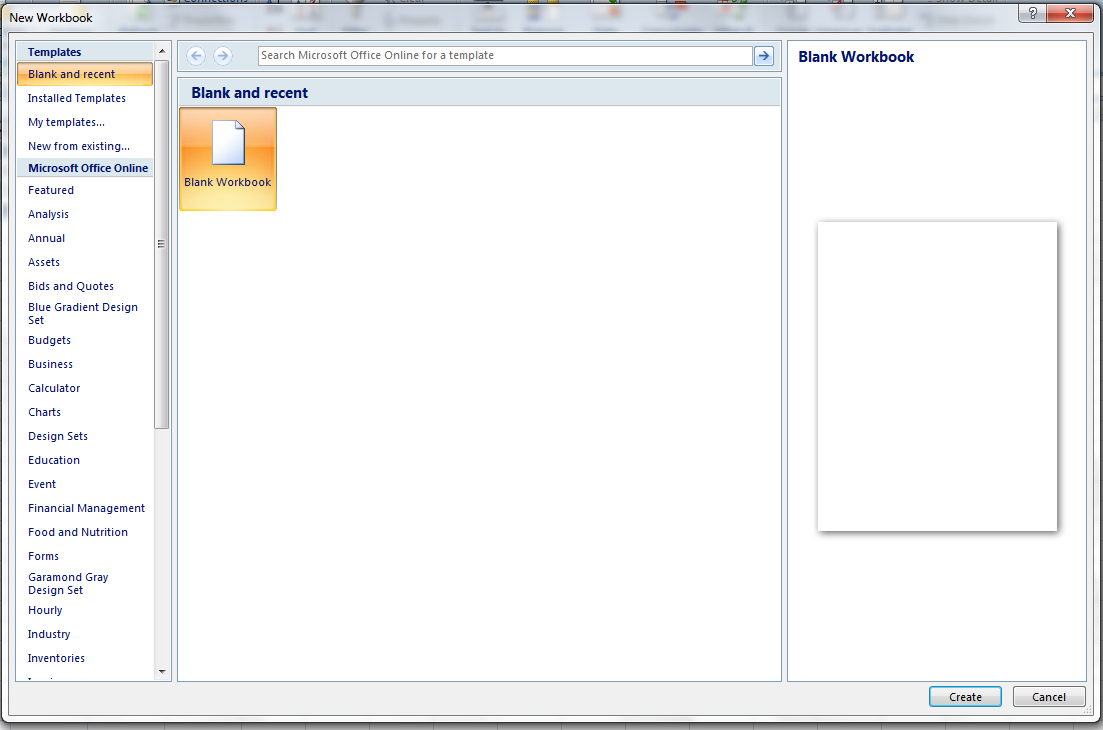
\includegraphics[scale=0.3]{src/images/chapter1_fig04.png}
\end{figure}

\section{वर्कबुक खोलना}\label{id-1.4}

किसी मौजूदा वर्कबुक को खोलने के लिए, आप निम्न चरणों का उपयोग सकते हैंः
\begin{descriptionSimple}{चरण 1:}
\item[चरण 1] \textbf{ऑफिस} बटन पर क्लिक करें और फिर \textbf{ओपन} क्लिक करें वैकल्पिक रूप से, ओपेन कमांड  {\rm (Ctrl+O)}  का उपयोग भी कर सकते हैं
\item[चरण 2] इच्छित वर्कबुक फ़ाइल को \textbf{ओपन डायलॉग} बॉक्स मे ढूँढें और डबल-क्लिक करे
\end{descriptionSimple}
\begin{figure}[H]
\centering
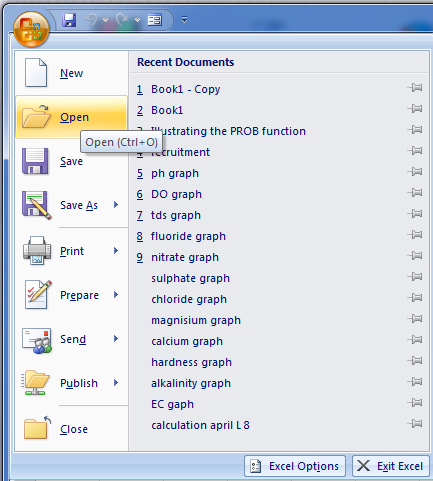
\includegraphics[scale=0.3]{src/images/chapter1_fig05.png}
\end{figure}
\begin{figure}[H]
\centering
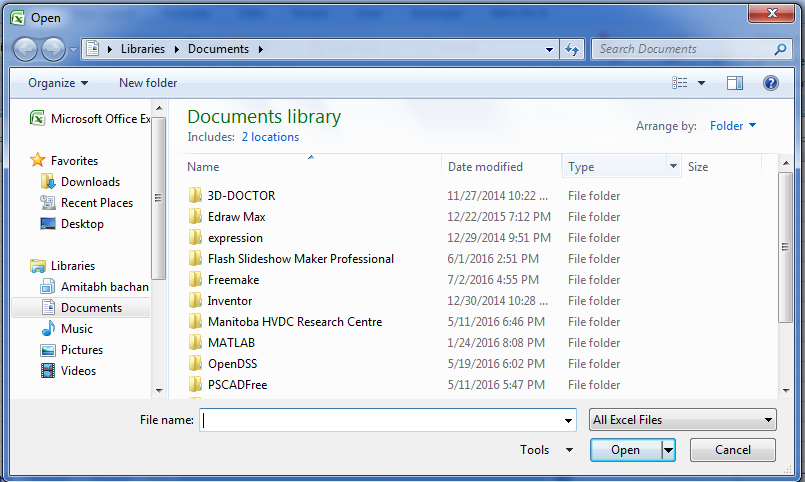
\includegraphics[scale=0.3]{src/images/chapter1_fig06.png}
\end{figure}

वैकल्पिक रूप से आप विंडो एक्सप्लोरर के लिए जा सकते हैं और जो फ़ाइल आप खोलना चाहते हैं उसका पता लगाकर उस पर डबल क्लिक करें ।

\section{लेबलिंग}\label{id-1.5}

कॉलम और रो शीर्षक (हेडिंग) के अक्षर और संख्याओं को लेबल कहा जाता है जो क्रमशः वर्कशीट के शीर्ष और बाईं ओर ग्रे-बाक्स में, प्रदर्शित होते हैं। कॉलम हेडिंग, अनुवर्णिक वर्ण (अल्फाबेटिक कैरक्टर्स) से लेबल रहती हैं जो कॉलम {\rm A} के साथ शुरु होती हैं। रो हेडिंग, संख्या से लेबल रहती हैं जो रो {\rm 1} के साथ शुरु होती हैं। आम तौर पर एक वर्कबुक {\rm Sheet1, Sheet2} और {\rm Sheet3} के रूप में तीन वर्कशीट द्वारा लेबल होती हैं। शीट का नाम बदलकर, नई शीट सम्मिलित करकेे, शीटों को हटाकर और मर्ज करके आप वर्कशीटो की लेबलिंग को बदल सकते हैं।

\section{वर्कबुक टैब्स को फॅार्मेट करना}\label{id-1.6}

जब आप एक नई वर्कबुक को खोलते हैं, या कोई मौजूदा वर्कबुक मे नई वर्कशीट जोडते है तब एक्सेल प्रत्येक शीट के लिए एक जेनेरिक नाम जैसे  {\rm Sheet1, Sheet2, Sheet3}  और इसी तरह, का उपयोग करता है। आप जैसे जैसे एक वर्कबुक का निर्माण करते है, आपको चीजें व्यवस्थित रखने के लिए इन शीटो का नाम बदलने की आवश्यकता होती है। एक वर्कशीट का नाम बदलने के लिए, सबसे आसान तरीका है कि इसके नाम पर डबल-क्लिक करें। यह नाम के टेक्स्ट को हाइलाइट कर देगा, और आप उसके बाद एक नया नाम टाइप कर सकते हैं। इसके अलावा भी, आप किसी वर्कशीट पर दायाँ क्लिक करके, पॉप-अप मेनू से रिनेम का चयन कर सकते हैं। टैब्स का नाम बदलने के कुछ नियम होते हैं। एक्सेल वर्कशीट का नाम कम से कम एक वर्ण (केरैक्टर) लंबा और 31 वर्णों से अधिक नहीं हो सकता। एक ही वर्कबुक में समान नाम के साथ दो शीटे नही हो सकती।

वर्कशीट नाम मे, प्रश्न चिह्न (क्वेश्चन मार्क्स), वर्ग कोष्ठक (स्क्वायर ब्रैकेट्स), तारक, अपोसट्रोफि, आगे और पीछे स्लैश (फॉरवर्ड एंड बैकवर्ड सलैशेस), अवधि (पीरियड्स) और कॅालन के रूप में कुछ वर्णों की अनुमति नहीं होती है। आप एक वर्कशीट टैब का रंग भी परिवर्तित कर सकते हैं। रंग बदलने के लिए, राइट क्लिक करें और मेनू से कलर टैब चुनें, और फिर अपनी पसंद का एक रंग चुनें।
\begin{figure}[H]
\centering

\includegraphics[scale=0.5]{src/images/chapter1_fig07.png}
\end{figure}

\section{वर्कशीट का स्थान बदलना (रिपोसिशन शीट्स)}\label{id-1.7}

एक वर्कबुक में, एक संपूर्ण वर्कशीट को किसी अन्य स्थान पर आसानी से मूव (ले जाना) या कॅापी (कॉपी बनाना) किया जा सकता हैं। परिकलन (कैलकुलेशन) या चार्ट्स का डेटा, वर्कशीट को ले जाने के दौरान गलत हो सकता है। शीट की स्थिति बदलने के लिए निम्न चरणों का पालन करेः
\begin{descriptionSimple}{चरण 1:}
\item[चरण 1] इच्छित वर्कशीटो का चयन करें जिसको आप मूव या कॅापी करना चाहते हैं
\item[चरण 2] \textbf{होम} टैब पर, \textbf{सेल} ग्रुप में, \textbf{फॉर्मेट} क्लिक करें, और फिर \textbf{ओर्गेनाइज शीटस्} के तहत \textbf{मूव आर कॅापी शीट} क्लिक करें\\  वैकल्पिक रूप से, आप दायाँ क्लिक करें और पॉप-अप मेनू से \textbf{मूव आर कॅापी} का चयन करें
\item[चरण 3] \textbf{मूव आर कॅापी} डायलाग बॉक्स में, \textbf{विफोर शीट लिस्ट} में, निम्न में से एक कार्य करेःं
	\begin{itemize}
		\item इच्छित षीट पर क्लिक करें जिसके पहले आप मूव या कॅापीड षीट को सम्मिलित करना चाहते है
		\item मूव या कॅापीड षीट को, वर्कबुक मे अंतिम षीट के बाद और \textbf{इन्सर्ट वर्कशीट} टैब से पहले ले जाने के लिए \textbf{मूव टु एन्ड} क्लिक करें
	\end{itemize}
\item[चरण 4] शीट को मूव के बजाय, कॅापी करने के लिए, \textbf{मूव आर कॅापी} डायलाग बॉक्स में \textbf{क्रिएट ए कॅापी} चेक बॉक्स का चयन करें
\end{descriptionSimple}

\begin{figure}[H]
\centering
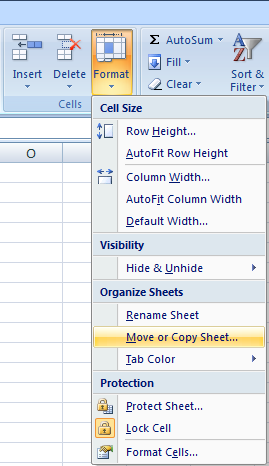
\includegraphics[scale=0.3]{src/images/chapter1_fig08.png}
\end{figure}
\begin{figure}[H]
\centering
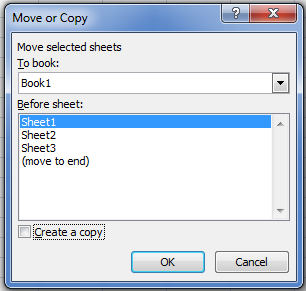
\includegraphics[scale=0.6]{src/images/chapter1_fig09.png}
\end{figure}

जब आप वर्कशीट की कॉपी बनाएँ, वर्कबुक में वह वर्कशीट दोहराइ जाती है, और शीट नाम दर्शाता है कि यह एक कॉपी हैं। उदाहरण के लिए, आप  {\rm Sheet1}  कि पहले कॉपी बनायेगें तब उसका नाम  {\rm Sheet1(2)}  होगा। हम वर्कशीटो को किसी अन्य वर्कबुक में भी मूव या कॅापी कर सकते हैं। इसके लिए, हमे यह सुनिश्चित करने की जरूरत है कि लक्ष्य (टारगेट) वर्कबुक एमएस एक्सेल की उसी आवृत्ति (इंस्टैंस) में खुली है। ऊपर की तरह अन्य सभी चरण समान हैं सिवाय \textbf{मूव आर कॅापी} डायलाग बॉक्स में, \textbf{टु बुक} सूची से उस वर्कबुक का चयन करें जिसमें आप चयनित शीटों को या उनकी कॉपी बनाकर ले जाना चाहते हैं

\section{वर्कशीट का नामकरण}\label{id-1.8}

किसी वर्कशीट का नामकरण (या नाम बदलने के लिए) निम्न चरणों का पालन करेः
\begin{descriptionSimple}{चरण 1:}
\item[चरण 1] इच्छित वर्कशीट टैब पर दायाँ क्लिक करें, जिसका आप नाम बदला चाहते है
\item[चरण 2] पॉप-अप मेनू से \textbf{रिनेम} का चयन करें
\item[चरण 3] नया नाम टाइप करें और  {\rm ENTER}  दबाएँ (हमारे उदाहरण में अनिल)
\end{descriptionSimple}

\begin{figure}[H]
\centering
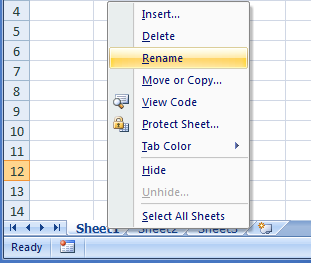
\includegraphics[scale=0.4]{src/images/chapter1_fig10.png}
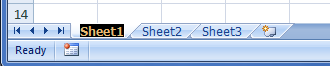
\includegraphics[scale=0.4]{src/images/chapter1_fig11.png}
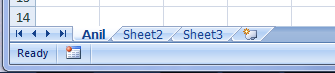
\includegraphics[scale=0.4]{src/images/chapter1_fig12.png}
\end{figure}

\section{वर्कशीट को जोड़ना}\label{id-1.9}

मौजूदा वर्कशीट के अंत में एक नए वर्कशीट को जोड़ने के लिए, स्क्रीन के नीचे, इन्सर्ट वर्कशीट टैब क्लिक करें। एक मौजूदा वर्कशीट के पहले, एक नई वर्कशीट इन्सर्ट (सम्मिलित) करने के लिए निम्न चरणों का पालन करेः
\begin{descriptionSimple}{चरण 1:}
\item[चरण 1] उस वर्कशीट टैब पर दायाँ क्लिक करें जिसके पहले आप एक नई वर्कशीट जोड़ना चाहते है
\item[चरण 2] पॉप-अप मेनू से \textbf{इन्सर्ट} का चयन करें
\end{descriptionSimple}		

\begin{figure}[H]
\centering
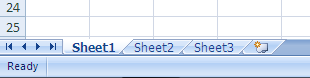
\includegraphics[scale=0.4]{src/images/chapter1_fig13.png}
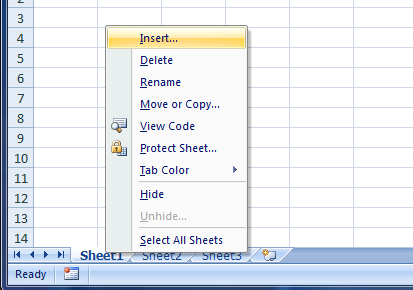
\includegraphics[scale=0.4]{src/images/chapter1_fig14.png}
\end{figure}

एक मौजूदा वर्कशीट के पहले एक नई वर्कशीट सम्मिलित करने के लिए, एक और तरीका निम्न~हैः
\begin{descriptionSimple}{चरण 1:}
\item[चरण 1] उस वर्कशीट टैब का चयन करें जिसके पहले आप एक नई वर्कशीट जोड़ना चाहते है
\item[चरण 2] \textbf{होम} टैब का चयन करें
\item[चरण 3] \textbf{सेलस्} ग्रुप में इन्सर्ट करें क्लिक करें
\item[चरण 4] \textbf{इन्सर्ट शीट} क्लिक करें
\end{descriptionSimple}

\begin{figure}[H]
\centering
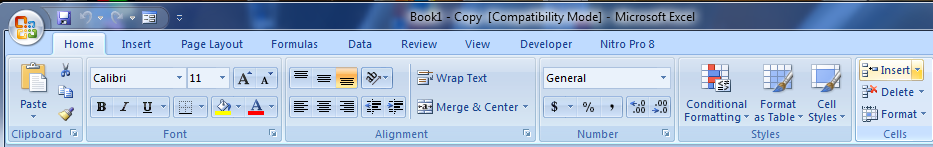
\includegraphics[scale=0.43]{src/images/chapter1_fig15.png}\\[5pt]
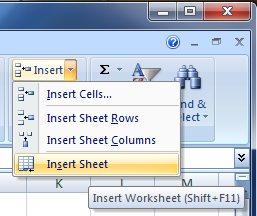
\includegraphics[scale=0.55]{src/images/chapter1_fig16.png}
\end{figure}

\section{वर्कशीट को हटाना}\label{id-1.10}			

किसी वर्कशीट को हटाने (डिलीट) के लिए, आप स्क्रीन के नीचे, उस वर्कशीट टैब पर दायाँ क्लिक करें जिसे आप हटाना चाहते हैं और पॉप-अप मेनू से \textbf{डिलीट} का चयन करें।

\begin{figure}[H]
\centering
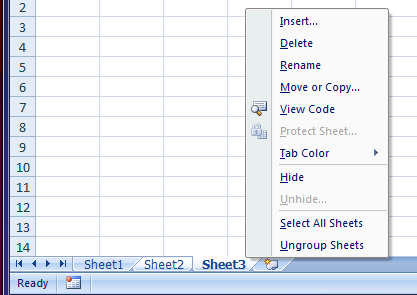
\includegraphics[scale=0.4]{src/images/chapter1_fig17.png}
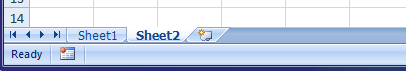
\includegraphics[scale=0.4]{src/images/chapter1_fig18.png}
\end{figure}

किसी वर्कशीट को हटाने के लिए एक और तरीकाः
\begin{descriptionSimple}{चरण 1:}
\item[चरण 1] वर्कशीट टैब का चयन करें जिसे आप हटाना चाहते हैं
\item[चरण 2] \textbf{होम} टैब का चयन करें
\item[चरण 3] \textbf{सेलस्} ग्रुप में \textbf{डिलीट} क्लिक करें
\item[चरण 4] \textbf{डिलीट शीट} पर क्लिक करें
\end{descriptionSimple}				
\begin{figure}[H]
\centering
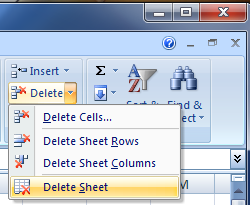
\includegraphics[scale=0.6]{src/images/chapter1_fig19.png}
\end{figure}

\section{वर्कशीट को छुपाना}\label{id-1.11}

किसी वर्कशीट को छुपाने (हाइड) के लिए, आप स्क्रीन के नीचे, वर्कशीट टैब पर दायाँ क्लिक करें जिसे आप छुपाना चाहते हैं और पॉप-अप मेनू से \textbf{हाइड} का चयन करें।

\begin{figure}[H]
\centering
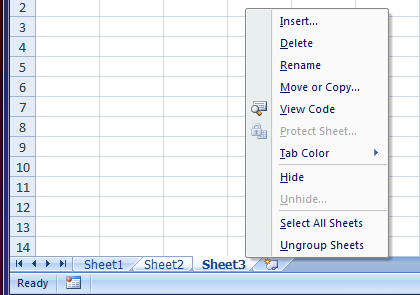
\includegraphics[scale=0.33]{src/images/chapter1_fig20.png}\qquad
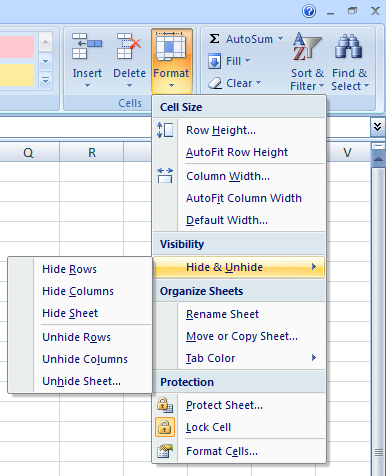
\includegraphics[scale=0.33]{src/images/chapter1_fig21.png}
\end{figure}

किसी वर्कशीट को छुपाने के लिए एक और तरीकाः		
\begin{descriptionSimple}{चरण 1:}
\item[चरण 1] वर्कशीट टैब का चयन करें जिसे आप छुपाना चाहते हैं
\item[चरण 2] \textbf{होम} टैब का चयन करें
\item[चरण 3] \textbf{सेलस्} ग्रुप में \textbf{फार्मेट} क्लिक करें
\item[चरण 4] \textbf{विजिबिलिटी} के तहत, \textbf{हाईड - अनहाईड} विकल्प पर जाएँ, और फिर \textbf{हाईड शीट} क्लिक करें
\end{descriptionSimple}
	
\section{वर्कशीट को दर्शाना (अनहाइड)}\label{id-1.12}

छुपी हुई वर्कशीट को दिखाने (अनहाइड) के लिए, निम्न चरणों का पालन करेः
\begin{descriptionSimple}{चरण 1:}
\item[चरण 1] वर्कशीट टैब पर दायाँ क्लिक करें
\item[चरण 2] पॉप-अप मेनू से \textbf{अनहाइड} का चयन करें
\item[चरण 3] सूची मे से सामने लाने वाली इच्छित वर्कशीटो का चयन करें और ओके क्लिक करें
\end{descriptionSimple}					

किसी वर्कशीट को लाने के लिए एक और तरीकाः
\begin{descriptionSimple}{चरण 1:}
\item[चरण 1] वर्कशीट टैब का चयन करें
\item[चरण 2] \textbf{होम} टैब का चयन करें
\item[चरण 3] \textbf{सेलस्} ग्रुप में \textbf{फार्मेट} क्लिक करें
\item[चरण 4] \textbf{विजिबिलिटी} के तहत, \textbf{हाईड - अनहाईड} विकल्प पर जाएँ, और फिर \textbf{अनहाईड शीट} क्लिक करें
\item[चरण 5] सूची मे से सामने लाने वाली इच्छित वर्कशीटो का चयन करें और ओके क्लिक करें
\end{descriptionSimple}
\newpage

\begin{figure}[t]
\centering
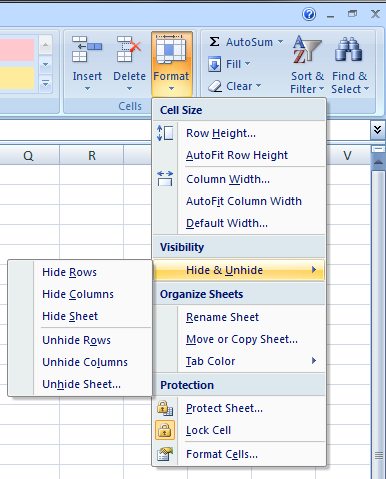
\includegraphics[scale=0.33]{src/images/chapter1_fig22.png}\qquad
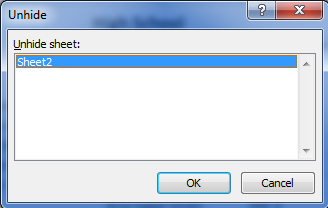
\includegraphics[scale=0.33]{src/images/chapter1_fig23.png}
\end{figure}

\section{वर्कबुक और वर्कशीटो को सहेजना (सेव करना)}\label{id-1.13}

आप किसी वर्कबुक को पहली बार सहेजने (सेव) के लिए, निम्नलिखित चरणों का उपयोग करेः
\begin{descriptionSimple}{चरण 1:}
\item[चरण 1] \textbf{ऑफिस} बटन पर क्लिक करें और फिर \textbf{सेव} क्लिक करें
\item[चरण 2] डायलॉग बॉक्स में, वह स्थान जहाँ आप फाइल को सहेजना चाहते हैं, का चयन करें
\item[चरण 3] फाइल का नाम टाइप करें
\item[चरण 4] \textbf{सेव} पर क्लिक करें
\end{descriptionSimple}

वैकल्पिक रूप से एक वर्कबुक ऊपरी बाएँ कोने में \textbf{सेव} चिह्न पर क्लिक करके या ( {\rm Ctrl+S} ) कमांड का उपयोग करके, सहेजा जा सकता हैं।

\begin{figure}[H]
\centering
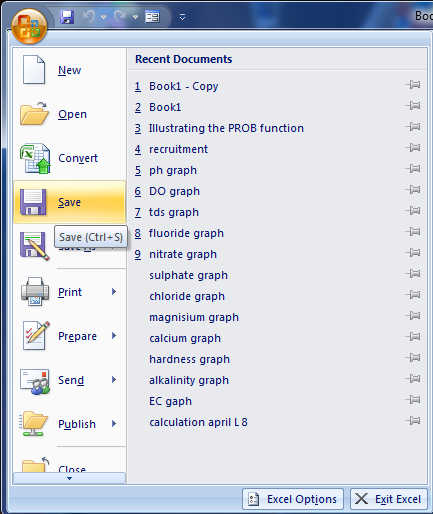
\includegraphics[scale=0.4]{src/images/chapter1_fig24.png}
\end{figure}
\begin{figure}[H]
\centering
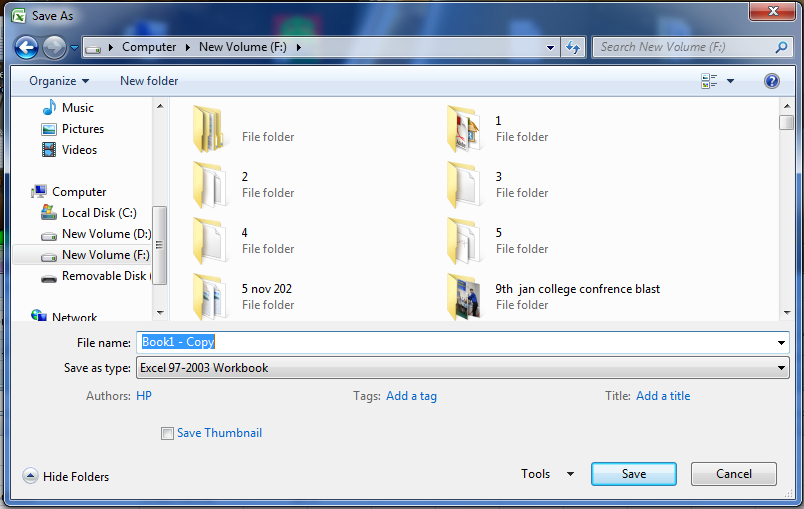
\includegraphics[scale=0.3]{src/images/chapter1_fig25.png}
\end{figure}

एक वर्कबुक बंद करने के लिए, \textbf{ऑफिस} बटन पर क्लिक करें, और उसके बाद \textbf{क्लोज} क्लिक करें.				

\begin{figure}[H]
\centering
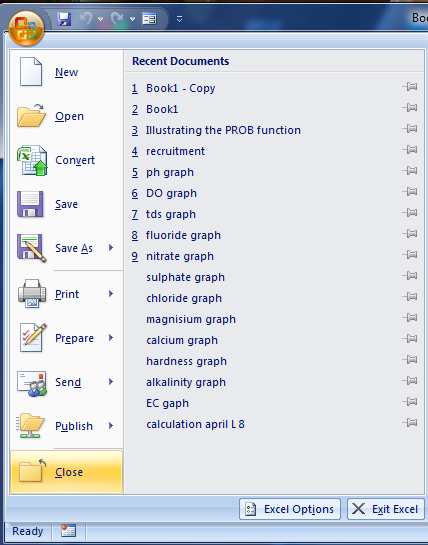
\includegraphics[scale=0.3]{src/images/chapter1_fig26.png}
\end{figure}				

\section{वर्कशीट में नेविगेट करना}\label{id-1.14}

किसी एक्सेल दस्तावेज मे जिसमे बहुत सारी वर्कशीटे होती हैं, उसमे चारों ओर नेविगेट (भ्रमण) करना मुश्किल हो सकता है। वर्तमान (करेंट) वर्कबुक में, जल्दी से एक अलग वर्कशीट पर पहुचने के लिए नेविगेशन बटन का उपयोग किया जा सकता हैं। एक्सेल वर्कबुक के निचले-बाएँ कोने में, आप वर्कशीट टैब के बाईं ओर चार नेविगेशन बटन देखेंगे।

\begin{figure}[H]
\centering
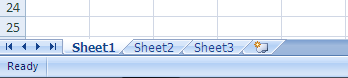
\includegraphics[scale=0.45]{src/images/chapter1_fig27.png}
\end{figure}

इन बटन पर राइट-क्लिक करने पर वर्तमान वर्कबुक में सभी वर्कशीटो की एक सूची प्रदर्शित करेगा, जिनकी पहचान उनके नाम द्वारा की जा सकती हैं। इस सूची में एक नाम का चयन करके आप उस वर्कशीट पर पहॅुच सकते हैं। वर्कबुक को नेवीगेट करने के लिए निम्न शॉर्टकट कुंजियाँ हैंः
\begin{itemize}[topsep=-1ex,parsep=0ex,partopsep=0ex,itemsep=0.5ex]
\item  {\rm Ctrl + Page Down:}  वर्कबुक में अगले शीट पर ले जाएगा
\item  {\rm Ctrl + Page Up:}  वर्कबुक में पिछले शीट पर ले जाएगा
\item  {\rm Ctrl + F6/ Tab:}  अगली वर्कबुक विंडो पर ले जाएगा
\item  {\rm Ctrl + Shift + F6/ Tab:}  पिछली वर्कबुक विंडो पर ले जाएगा
\item  {\rm F6 / Shift + F6:}  एक वर्कशीट जो कि विभाजित कि गयी है, उसके अगले/पिछले वर्कशीट-पैन पर ले जाएगा			
\end{itemize}
				
\section{सेल, रो या/और कॉलम को सम्मिलित करना}\label{id-1.15}

\paragraphTitle{किसी वर्कशीट में रिक्त सेल को सम्मिलित करना}

उस सेल का चयन करें, जहाँ आप नई रिक्त सेल सम्मिलित (इन्सर्ट) करना चाहते हैं और निम्न चरणों का उपयोग करेः
\begin{descriptionSimple}{चरण 1:}
\item[चरण 1] \textbf{होम} टैब पर, \textbf{सेलस्} ग्रुप में, \textbf{इन्सर्ट} क्लिक करें
\item[चरण 2] \textbf{इन्सर्ट सेलस्} क्लिक करें\\  आप चयनित सेल पर राइट-क्लिक करके और फिर \textbf{इन्सर्ट} को क्लिक करके भी यह काम कर सकते हैं
\item[चरण 3] \textbf{इन्सर्ट डॅायलाग} बॉक्स में, उपयुक्त विकल्प का चयन करें
\end{descriptionSimple}
\begin{figure}[H]
\centering
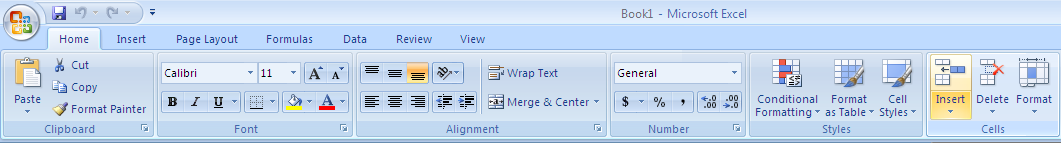
\includegraphics[scale=0.33]{src/images/chapter1_fig28.png}\\[4pt]
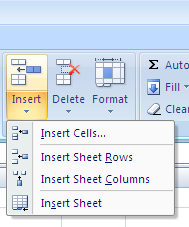
\includegraphics[scale=0.4]{src/images/chapter1_fig29.png}\qquad
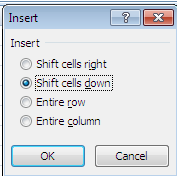
\includegraphics[scale=0.4]{src/images/chapter1_fig30.png}
\end{figure}

एक से अधिक सेलो को इन्सर्ट करने के लिए, वर्कशीट में जहाँ आप नई रिक्त सेलों को इन्सर्ट करना चाहते हैं, वहॅा एक से अधिक सेलों का चयन करें और फिर उपर दिये गये चरणों का पालन करे। उदाहरण के लिए, चार रिक्त सेलों को इन्सर्ट करने के लिए, आपको चार सेलों का चयन करने की जरूरत है।

\paragraphTitle{वर्कशीट में रिक्त रो को सम्मिलित करना}
\begin{descriptionSimple}{चरण 1:}
\item[चरण 1]
		\begin{itemize}
		\item एक रो को इन्सर्ट करने के लिए, रो या रो में से एक सेल का चयन करें, जिसके उपर आप नए रिक्त रो को इन्सर्ट करना चाहते हैं
		\item एक से अधिक रो को इन्सर्ट करने के लिए, रो का चयन करें, जिसके उपर आप नए रिक्त रो को इन्सर्ट करना चाहते हैं (असन्निकट (नॉन-अड़जसेन्ट) रो को इन्सर्ट करने के लिये, आप असन्निकट रो का चयन करते समय ब्जतस दबाए रखें)		\end{itemize}
\item[चरण 2] \textbf{होम} टैब पर, \textbf{सेलस्} ग्रुप में, \textbf{इन्सर्ट} क्लिक करें
\item[चरण 3] \textbf{इन्सर्ट शीट रोज} क्लिक करें\\ आप चयनित रो पर राइट-क्लिक करें और फिर \textbf{इन्सर्ट} क्लिक करकें भी आप यह काम कर सकते हैं।
\end{descriptionSimple}
\begin{figure}[H]
\centering
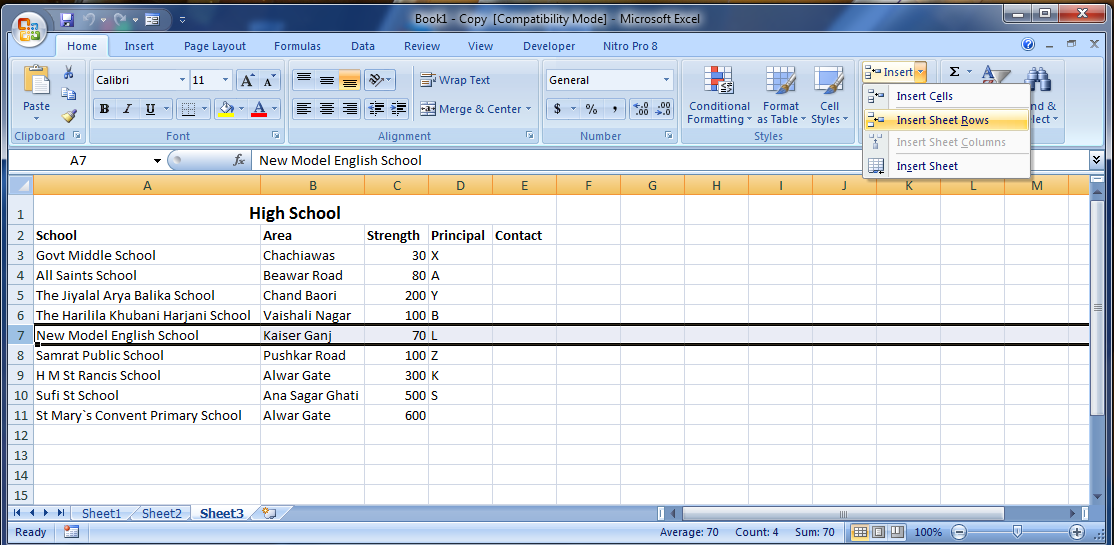
\includegraphics[scale=0.33]{src/images/chapter1_fig31.png}
\end{figure}

\paragraphTitle{वर्कशीट में रिक्त कॉलम सम्मिलित करना}
\begin{descriptionSimple}{चरण 1:}
\item[चरण 1]
		\begin{itemize}
		\item एक कॉलम को इन्सर्ट करने के लिए, कॉलम या कॉलम में से एक सेल का चयन करें, जिसके तुरंत दाएँ आप नए रिक्त कॉलम को इन्सर्ट करना चाहते हैं
		\item एक से अधिक कॉलमो को इन्सर्ट करने के लिए, कॉलमो का चयन करें, जिसके तुरंत दाएँ नए रिक्त कॉलमो को इन्सर्ट करना चाहते हैं (असन्निकट (नॉन-अड़जसेन्ट) कॉलमो को इन्सर्ट करने के लिये, आप असन्निकट कॉलमो का चयन करते समय  {\rm Ctrl}  दबाए रखें)
		\end{itemize}
\item[चरण 2] \textbf{होम} टैब पर, \textbf{सेलस्} ग्रुप में, \textbf{इन्सर्ट} क्लिक करें
\item[चरण 3] \textbf{इन्सर्ट शीट कॉलम} क्लिक करें\\  आप चयनित कॉलम (कॉलमो) पर राइट-क्लिक करें और फिर \textbf{इन्सर्ट} क्लिक करकें भी आप यह काम कर सकते हैं।
\end{descriptionSimple}
\begin{figure}[H]
\centering
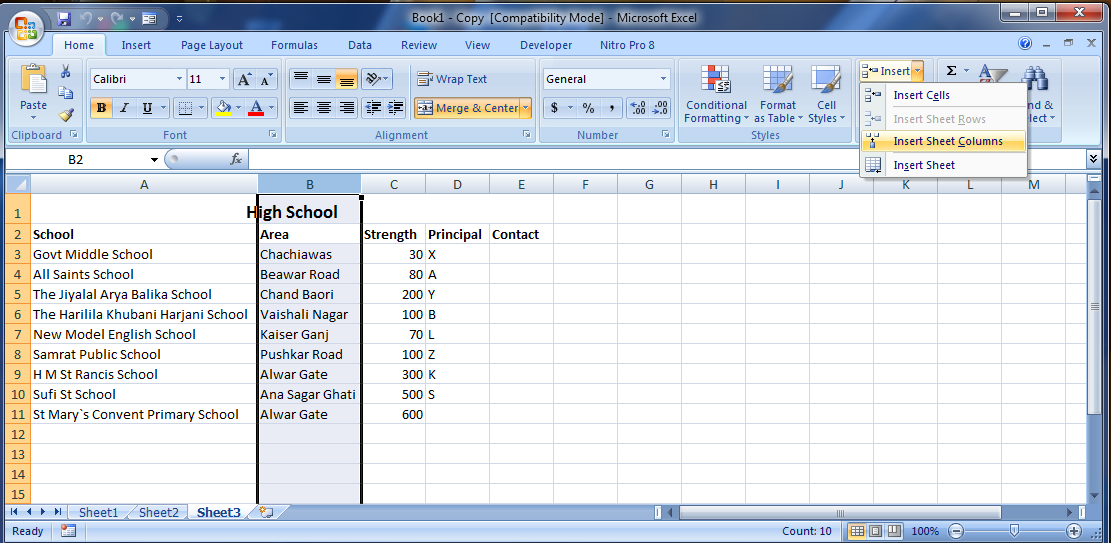
\includegraphics[scale=0.33]{src/images/chapter1_fig32.png}
\end{figure}

\section{सेलों, रो या कॉलमो को हटाना}\label{id-1.16}	

इच्छित सेलों, रो, कॉलमो का चयन करें जिसको आप हटाना चाहते है और निम्न चरणों का पालन करेः
\begin{descriptionSimple}{चरण 1:}
\item[चरण 1] \textbf{होम} टैब पर, \textbf{सेलस्} ग्रुप में, \textbf{डिलीट} क्लिक करें
\item[चरण 2]
		\begin{itemize}
		\item चयनित सेलों को हटाने के लिए, \textbf{डिलीट सेल} क्लिक करें
		\item चयनित रो को हटाने के लिए, \textbf{डिलीट शीट रोज} क्लिक करें
		\item चयनित कॉलमो को हटाने के लिए, \textbf{डिलीट शीट कॉलम} क्लिक करें
		\end{itemize}
\item[चरण 3] \textbf{डिलीट} डायलाग बॉक्स में, उपयुक्त विकल्प का चयन करें
\end{descriptionSimple}
\begin{figure}[H]
\centering
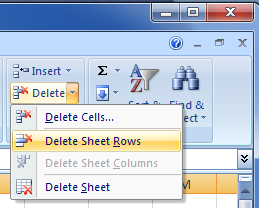
\includegraphics[scale=0.5]{src/images/chapter1_fig33.png}\qquad
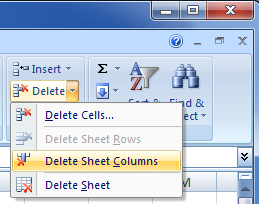
\includegraphics[scale=0.5]{src/images/chapter1_fig34.png}
\end{figure}

आप चयनित सेलों, रो, कॉलमस् पर राइट-क्लिक करें और फिर डिलीट क्लिक करकें भी आप यह काम कर सकते हैं।

	
\section{सेलो को विलय करना}\label{id-1.17}

सेल विलय (मर्ज), चयनित सेलों को एक सेल में कनवर्ट करता है। यह शीर्षक बनाने के लिए उपयोगी हो सकता है। आप दो या दो से अधिक सेलों से टेक्स्ट को एक सेल में मर्ज या संयोजित कर सकते हैं। मर्ज करने के लिए निम्न चरणों का उपयोग करेंः

\begin{descriptionSimple}{चरण 1:}
\item[चरण 1]  आप जिन्हे मर्ज करना चाहते हैं उन सेलों का चयन करें
\item[चरण 2] \textbf{होम} टैब के \textbf{एलाइनमेंट} ग्रुप मे जाए
\item[चरण 3] \textbf{मर्ज - सेण्टर} क्लिक करें\\  यहॅा चार विकल्प है:
		\begin{itemize}
		\item मर्ज - सेण्टर
		\item मर्ज अक्रॉस
		\item मर्ज सेलस्
		\item अनमर्ज सेल
		\end{itemize}
\item[चरण 4]  उपयुक्त विकल्प क्लिक करें
\end{descriptionSimple}				
\begin{figure}[H]
\centering
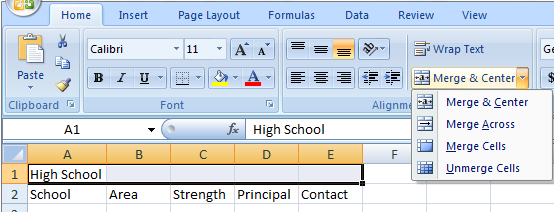
\includegraphics[scale=0.4]{src/images/chapter1_fig35.png}\qquad
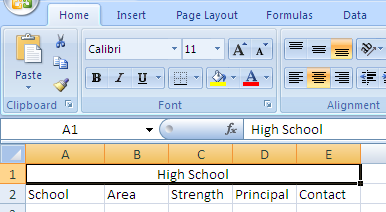
\includegraphics[scale=0.4]{src/images/chapter1_fig36.png}
\end{figure}
				
\section{सेलो को विभाजित करना}\label{id-1.18}

सेलों को मर्ज करने के बाद, आप मर्ज किए गए सेल को अलग-अलग सेलों में फिर से विभाजित (स्प्लिट) कर सकते हैं। आप किसी मर्ज न किए गए (अनमर्ज) सेल को विभाजित नहीं कर सकते हैं। विभाजन करने के लिए निम्न चरणों का उपयोग करेःं

\begin{descriptionSimple}{चचरण 1:}
\item[चचरण 1] आप जिन्हे विभाजित करना चाहते हैं उन सेलों का चयन करें
\item[चचरण 2] \textbf{होम} टैब के \textbf{एलाइनमेंट} ग्रुप में जाए
\item[चचरण 3] \textbf{मर्ज - सेण्टर} क्लिक करें
\item[चचरण 4] \textbf{अनमर्ज सेलस्} विकल्प को क्लिक करें
\end{descriptionSimple}
\begin{figure}[H]
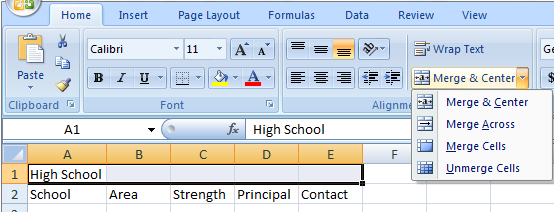
\includegraphics[scale=0.4]{src/images/chapter1_fig37.png}\qquad
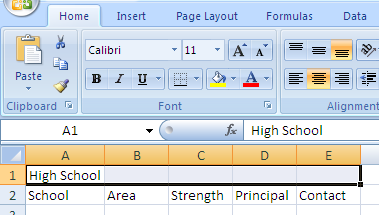
\includegraphics[scale=0.4]{src/images/chapter1_fig38.png}
\end{figure}					

\section{रो और कॉलम को छुपाना}\label{id-1.19}

कॉलम (कॉलमो) या रो छुपाने से आपको अपनी वर्कबुक में अवांछित परिवर्तन रोकने मेे मदद मिलेगी। रो/कॉलम को छुपाने के लिए, निम्न चरणों का उपयोग करेःं

\begin{descriptionSimple}{चरण 1:}
\item[चरण 1] इच्छित कॉलम/रो हेडर पर क्लिक कर उनका चयन करे, जिसे आप छुपाना चाहते है
\item[चरण 2] \textbf{होम} टैब पर, \textbf{सेलस्} ग्रुप में, \textbf{फार्मेट} क्लिक करें
\item[चरण 3] \textbf{विजिबिलिटी} के तहत, \textbf{हाईड \& अनहाईड} विकल्प पर जाएँ, और फिर \textbf{हाईड कॉलम/हाईड रो} को क्लिक करें
\end{descriptionSimple}
\begin{figure}[H]
\centering
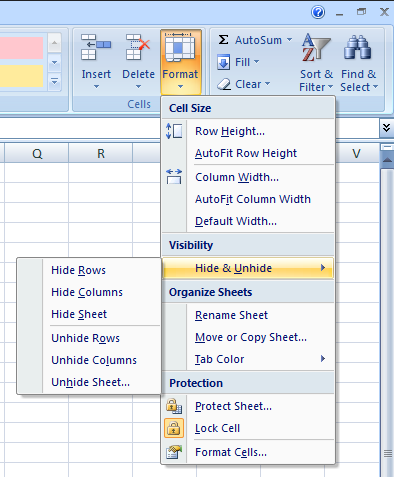
\includegraphics[scale=0.45]{src/images/chapter1_fig39.png}
\end{figure}				

आप चयनित रो, कॉलमो के हेडर पर राइट-क्लिक करें, और फिर \textbf{हाईड} क्लिक करकें भी आप यह काम कर सकते हैं।

\section{कॉलम और रो को दर्शाना}\label{id-1.20}

छुपे हुए रो/कॉलम को दर्शाने (अनहाइड) के लिए, निम्न चरणों का उपयोग करेंः

\begin{descriptionSimple}{चरण 1:}
\item[चरण 1] जिन कॉलम/रो को सामने लाना चाहते हैं उनके दोनों ओर से सटे कॉलम/रो का चयन करे
\item[चरण 2] \textbf{होम} टैब पर, \textbf{सेलस्} ग्रुप में, \textbf{फार्मेट} क्लिक करें
\item[चरण 3] \textbf{विजिबिलिटी} के तहत, \textbf{हाईड \& अनहाईड} विकल्प पर जाएँ, और फिर \textbf{अनहाईड कॉलम/अनहाईड रो} को क्लिक करें
\end{descriptionSimple}

आप चयनित रो, कॉलमो के हेडर पर राइट-क्लिक करें, और फिर अनहाईड क्लिक करकें भी आप यह काम कर सकते हैं।

									
\section{स्वरूपित करना}\label{id-1.21}

एक्सेल में, हर सेल को अलग ढंग से स्वरूपित (फार्मेट) कर सकते हैं। आपके एक्सेल वर्कबुक को अनुकूलित करने के लिए यहाँ कई विकल्प उपलब्ध हैं, जो आपकी वर्कशीट को पढ़ने के लिए आसान बना सकते हैं। एक्सेल कई संख्या स्वरूप (नंबर फार्मेट) प्रदान करता है, जिनसे आप अपने दस्तावेज मे संख्या कैसे दिखाई देगी का मानकीकरण कर सकते हैं। अगले अध्याय में विस्तार से इस विषय का वर्णन किया गया है। सेलों को फार्मेट करने के लिए निम्न चरणों का पालन करेःं

\begin{descriptionSimple}{चरण 1:}
\item[चरण 1] उन सेलों का चयन करें जिन्हे आप फार्मेट करना चाहते हैं
\item[चरण 2] राइट-क्लिक करें और फिर पॉपअप मेनू से \textbf{फार्मेट सेलस्} का चयन करें
\item[चरण 3] \textbf{फार्मेट सेलस्} से उपयुक्त विकल्प का चयन करें और ओके क्लिक करें
\end{descriptionSimple}
\begin{figure}[H]
\centering
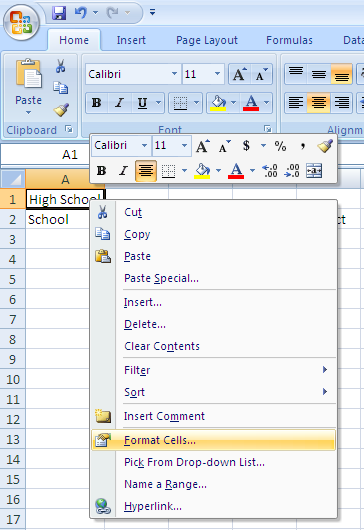
\includegraphics[scale=0.33]{src/images/chapter1_fig40.png}\qquad
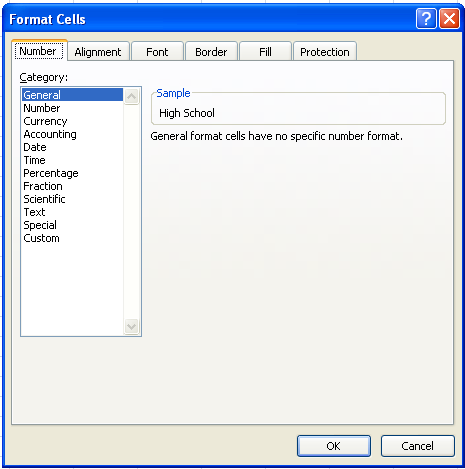
\includegraphics[scale=0.33]{src/images/chapter1_fig41.png}
\end{figure}								
	
\section{सेलों को फिल्टर और सॉर्ट करना}\label{id-1.22}

सॉर्ट (क्रमवार लगाना) एक सामान्य स्प्रेडशीट कार्य हैं जिससे आप आसानी से अपने डेटा को पुनः व्यवस्थित कर सकते हैं। सॉर्ट का सबसे आम प्रकार वर्णानुक्रम (अल्फाबेटिकल ऑर्डरिंग) सॉर्ट हैं, जिसे आप आरोही (असेंडिंग) या अवरोही (डिसेंडिंग) क्रम में कर सकते हैं है। वर्णानुक्रम में सॉर्ट करने के लिएः

\begin{descriptionSimple}{चरण 1:}
\item[चरण 1] इच्छित कॉलम में किसी सेल का चयन करें जिसको आप सॉर्ट करना चाहते है
\item[चरण 2] \textbf{होम} टैब के \textbf{एडिटिंग} ग्रुप मे \textbf{सॉर्ट \& फिल्टर} कमांड क्लिक करें
\item[चरण 3] उपयुक्त विकल्प का चयन करें
\end{descriptionSimple}
\begin{figure}[H]
\centering
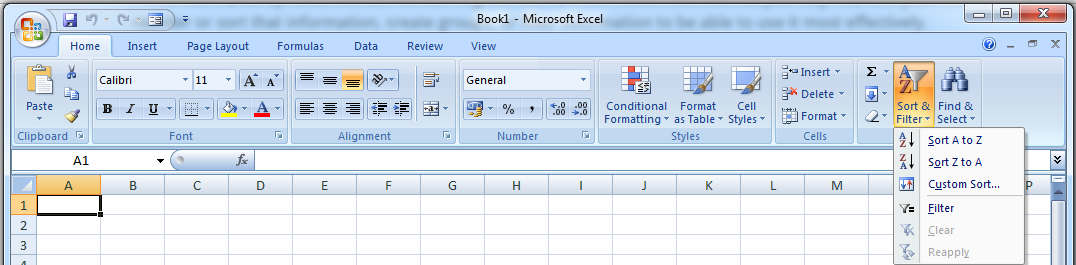
\includegraphics[scale=0.33]{src/images/chapter1_fig42.png}
\end{figure}

आप डेटा को फिल्टर (अलग करना) करके केवल उन्ही रो को प्रदर्शित कर सकते हैं जो आपके द्धारा निर्दिष्ट किये गये मापदंड से मेल खाती हैं, और उन रो को छुपा सकते हैं जिन्हे आप प्रदर्शित नहीं करना चाहते हैं। डेटा को फिल्टर करने के बाद, आप इसको कॉपी, फाइंड, एडिट, फॉर्मेट, चार्ट और फिल्टर किए हुए डेटा के सबसेट को बिना उलटफेर या मूव किए, प्रिंट कर सकते हैं। आप एक से अधिक कॉलम के अनुसार भी फिल्टर कर सकते हैं। फिल्टर योगात्मक होते हैं, जिसका अर्थ है कि प्रत्येक अतिरिक्त फिल्टर वर्तमान फिल्टर पर आधारित होता है और डेटा के सबसेट को आगे कम करता हैं।


\section{हैडर्स एंड फूटर्स}\label{id-1.23}

एक दस्तावेज की पहचान करने और उसे व्यवस्थित करने के लिए हैडर्स (शीर्ष लेख) और फूटर्स (पाद लेख) उपयोगी हो सकते है। हैडर जानकारी का वो भाग हैं, जो दस्तावेज के मुख्य भाग के ऊपर प्रिंट किया जाता है और फूटर जानकारी का वो भाग हैं, जो दस्तावेज के मुख्य भाग के नीचे प्रिंट किया जाता हैं। अक्सर हैडर्स और फूटर्स की जानकारी पूरे दस्तावेज में स्थिर रहती हैं। उदाहरण के लिए आप एक फूटर मे, पेज संख्या, दिनांक और समय, और आपकी फाइल का नाम बता सकते हैं। आप अपने दस्तावेज में किसी अंतर्निहित हैडर्स या फूटर्स को जोड़ सकते हैं, या एक कस्टम हैडर और फूटर बना सकते हैं। हैडर्स और फूटर्स केवल पेज लेआउट व्यू और मुद्रित (प्रिंटेड) पेजों पर प्रदर्शित होते हैं। वे साधारण (नार्मल) व्यू में वर्कशीट पर प्रदर्शित नहीं होते हैं। आप हैडर्स या फूटर्स को पेज लेआउट व्यू में इन्सर्ट कर सकते हैं, या यदि आप एक ही समय में एक से अधिक वर्कशीट पर हैडर्स या फूटर्स इन्सर्ट करना चाहते हैं, तो आप पेज सेटअप डायलाग बॉक्स का उपयोग कर सकते हैं।


पेज लेआउट व्यू में हैडर और फूटर के टेक्स्ट को जोड़ने या परिवर्तित करने के लिए निम्नलिखित चरणो का उपयोग करेः

\begin{descriptionSimple}{चरण 1:}
\item[चरण 1] उस वर्कशीट पर क्लिक करें जिसमें आप हैडर और फूटर जोड़ना चाहते हैं या जिसमें वे हैडर और फूटर हों जिसे आप परिवर्तित करना चाहते हैं
\item[चरण 2] \textbf{इंसर्ट टैब} पर, \textbf{टेक्स्ट ग्रुप} में, \textbf{हैडर और फूटर} पर क्लिक करे, एक्सल \textbf{पेज लेआउट} व्यू में वर्कशीट प्रदर्शित करेगा (आप इस व्यू को प्रदर्शित करने के लिए स्टैटस-बार पर \textbf{पेज लेआउट} व्यू भी क्लिक कर सकते हैं)
\item[चरण  3] निम्न में से कोई एक कार्य करेंः
			\begin{itemize}
			\item हैडर या फूटर जोड़ने के लिए वर्कशीट पेज के शीर्ष और निचले हिस्से में बाएँ, मध्य, या दाएँ हैडर या \textbf{फूटर टेक्स्ट} बॉक्स पर क्लिक करें
			\item हैडर या फूटर परिवर्तित करने के लिए, वर्कशीट पेज के शीर्ष और निचले हिस्से में बाएँ, मध्य, या दाएँ हैडर या फूटर टेक्स्ट बॉक्स पर क्लिक करें जिसमें हैडर या फूटर है। उसके बाद उस टेक्स्ट का चयन करें जिसे परिवर्तित किया जाना है
			\end{itemize}
\item[चरण 4] इच्छित टेक्स्ट लिखें
\end{descriptionSimple}

हैडर या फूटर बंद करने के लिए वर्कशीट में कहीं भी क्लिक करें (आपके द्वारा किए गए बदलावों को रखे बिना हैडर्स या फूटर्स बंद करने के लिए,  {\rm ESC}  दबाएँ )

पेज सेटअप डायलाग बॉक्स का उपयोग करके, हैडर और फूटर के टेक्स्ट को जोड़ने या परिवर्तित करने के लिए निम्नलिखित चरणो का उपयोग करेः
		
\begin{descriptionSimple}{चरण 1:}
\item[चरण 1] उस वर्कशीट पर क्लिक करे, जिसमें आप हैडर्स या फूटर्स को जोड़ना चाहते हैं या जिसमें वे हैडर और फूटर हों जिन्हे आप परिवर्तित करना चाहते हैं
\item[चरण 2] \textbf{पेज लेआउट} टैब पर, \textbf{पेज सेटअप} ग्रुप में, डायलाग बॉक्स लॉन्चर को क्लिक करे, \textbf{पेज सेटअप} डायलाग बॉक्स प्रदर्शित होगा
\item[चरण 3] \textbf{हैडर्स/फूटर्स} टैब पर, \textbf{कस्टम हैडर्स} या \textbf{कस्टम फूटर्स} पर क्लिक करें 
\item[चरण 4] \textbf{लेफ्ट सेक्शन, सेंटर सेक्शन,} या \textbf{राईट सेक्शन} बॉक्स में, इच्छित हैडर्स या फूटर्स की जानकारी इन्सर्ट करने के लिए उस सेक्शन बॉक्स में क्लिक करें
\item[चरण 5] हैडर्स या फूटर्स टेक्स्ट जोड़ने या परिवर्तित करने के लिए, \textbf{लेफ्ट सेक्शन, सेंटर सेक्शन,} या \textbf{राईट सेक्शन} बॉक्स में मौजूदा टेक्स्ट संपादित करें या अतिरिक्त टेक्स्ट लिखें
\end{descriptionSimple}	
\begin{figure}[H]
\centering
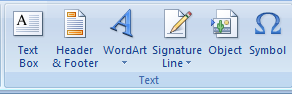
\includegraphics[scale=0.4]{src/images/chapter1_fig43.png}\qquad
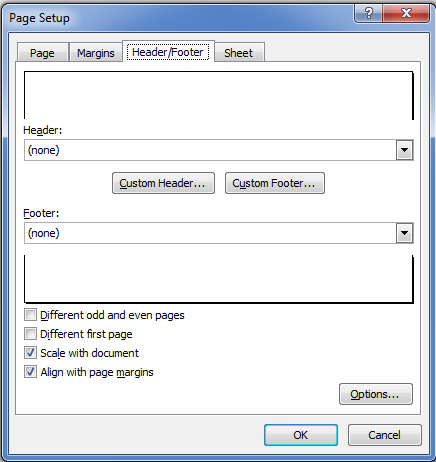
\includegraphics[scale=0.25]{src/images/chapter1_fig44.png}
\end{figure}
\begin{figure}[H]
\centering
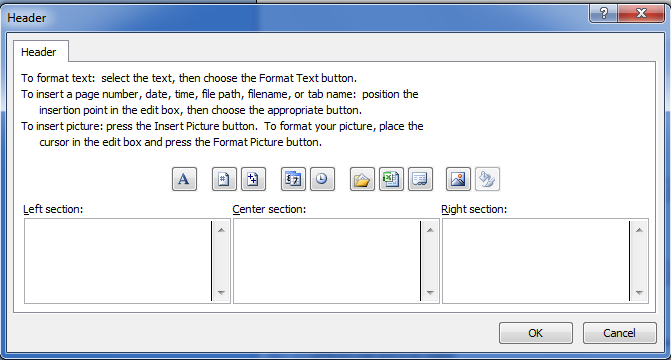
\includegraphics[scale=0.4]{src/images/chapter1_fig45.png}\\[4pt]
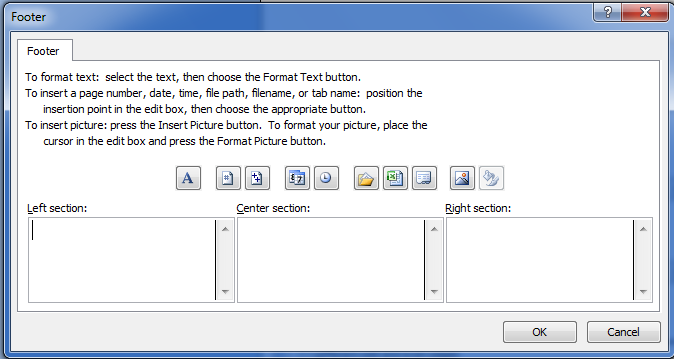
\includegraphics[scale=0.4]{src/images/chapter1_fig46.png}
\end{figure}
						
\section{हैडर्स और फूटर्स के लिए मार्जिन सेट करना}\label{id-1.24}

यदि आपके हैडर्स या फूटर्स के प्रदर्शन के साथ समस्याएँ हैं, तो आप मार्जिन (हाशिये) समायोजित करके उन्हें ठीक कर सकते हैं। आप दो तरीकों से मार्जिन समायोजित कर सकते हैंः माउस विकल्प या पेज सेटअप डायलाग बॉक्स विकल्प का उपयोग करके।


माउस के साथ मार्जिन को समायोजित करने के लिए निम्न चरणों का पालन करेःं

\begin{descriptionSimple}{चरण 1:}
\item[चरण 1] \textbf{ऑफिस} बटन से \textbf{प्रिंट} का चयन करें, और फिर \textbf{प्रिंट प्रीव्यू} क्लिक करें (दस्तावेज प्रिंट प्रीव्यू मोड में प्रदर्शित हो जाएगा)
\item[चरण 2] \textbf{प्रीव्यू} ग्रुप में, \textbf{शो मार्जिन} का चयन करें (मार्जिन रूपरेखा दिखाई देगी)
\item[चरण 3] माउस का उपयोग कर, मार्जिन रूपरेखा को क्लिक करें और इच्छित स्थान पर खींचें
\item[चरण 4] \textbf{क्लोज प्रिंट प्रीव्यू} क्लिक करें
\end{descriptionSimple}				
\begin{figure}[tbp]
\centering
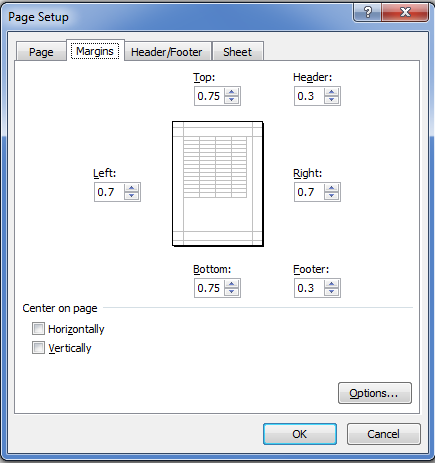
\includegraphics[scale=0.4]{src/images/chapter1_fig47.png}
\end{figure}

पेज सेटअप डायलाग बॉक्स के साथ मार्जिन को समायोजित करने के लिए निम्न चरणों का उपयोग करेःं

\begin{descriptionSimple}{चरण 1:}
\item[चरण 1] \textbf{ऑफिस} बटन मेनू से \textbf{प्रिंट} का चयन करें, और \textbf{प्रिंट प्रीव्यू} क्लिक करें (दस्तावेज प्रिंट प्रीव्यू मोड में प्रदर्शित हो जाएगा)
\item[चरण 2] \textbf{प्रिंट} ग्रुप में, पेज \textbf{सेटअप} क्लिक करें (\textbf{पेज सेटअप} डायलाग बॉक्स प्रदर्शित हो जाएगा)
\item[चरण 3] \textbf{मार्जिन} टैब का चयन करें
\item[चरण 4] टॉप, लेफ्ट, राईट, बॉटम, हैडर और/या फूटर टेक्स्ट बॉक्स में टाइप करें, पसंदीदा मार्जिन वैल्यू को दर्ज करें या मार्जिन समायोजित करने के लिए नज बटनों का उपयोग करें
\item[चरण 5] ओके क्लिक करें
\item[चरण 6] \textbf{क्लोज प्रिंट प्रीव्यू} क्लिक करें
\end{descriptionSimple}

\section{प्रिंटींग के बारे में जानकारी}\label{id-1.25}

आप एक समय में एक या एक बार में कई, आंशिक या पूरी वर्कशीटो और वर्कबुको को प्रिंट (मुद्रित) कर सकते हैं। और यदि आप जो डेटा प्रिंट करना चाहते हैं वह किसी माइक्रोसॉफ्ट ऑफिस एक्सेल टेबल में है, तो आप केवल एक्सेल टेबल प्रिंट कर सकते हैं। आप कोई वर्कबुक को किसी एक प्रिंटर के बजाय फाइल मे भी प्रिंट कर सकते हैं। एक आंशिक या संपूर्ण वर्कशीट या वर्कबुक को प्रिंट करने के लिए निम्न चरणों का पालन करेः

\begin{descriptionSimple}{चरण 1}
\item[चरण 1] निम्न में से एक करेंः
			\begin{itemize}
			\item एक आंशिक वर्कशीट को प्रिंट करने के लिए, वर्कशीट पर क्लिक करें, और उसके बाद प्रिंट करने के लिए इच्छित डेटा की रेंज का चयन करें
			\item संपूर्ण वर्कशीट प्रिंट करने के लिए, उस वर्कशीट को क्लिक करके उसे सक्रिय (एक्टिव) बनाए
			\item किसी वर्कबुक को प्रिंट करने के लिए, इसकी किसी भी वर्कशीट को क्लिक करें
			\end{itemize}
\item[चरण 2] \textbf{ऑफिस} बटन क्लिक करें और फिर \textbf{प्रिंट} क्लिक करें (या शॉर्टकट कमांड  {\rm Ctrl + P}  दबाएँ), प्रिंट डायलाग बॉक्स प्रदर्शित किया जाएगा
\item[चरण 3] \textbf{प्रिंट वाट} अनुभाग के तहत, चयन, एक्टिव शीट या शीटो या संपूर्ण वर्कबुक प्रिंट करने के लिए, एक विकल्प का चयन करें
\item[चरण 4] \textbf{कॉपीज} अनुभाग के तहत, आप प्रिंट के लिए कॉपीयों की संख्या निर्दिष्ट कर सकते हैं
\end{descriptionSimple}
\begin{figure}[H]
\centering
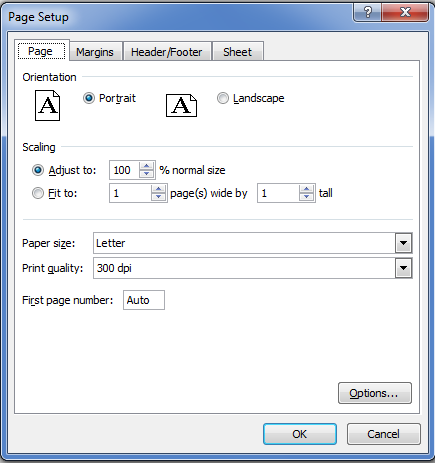
\includegraphics[scale=0.35]{src/images/chapter1_fig48.png}\qquad
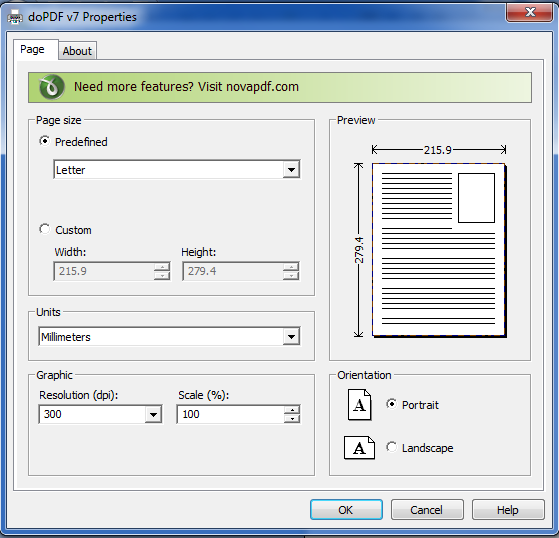
\includegraphics[scale=0.35]{src/images/chapter1_fig49.png}
\end{figure}
	
\section{प्रिंट एरिया का चयन करना}\label{id-1.26}

यदि आप अक्सर वर्कशीट पर एक विशेष चयन (सेलेक्सन) प्रिंट करते है तो आप एक प्रिंट एरिया (क्षेत्र) निर्धारित कर सकते हैं, जो बस उस चयन को शामिल करे। जब आप कोई प्रिंट एरिया निर्धारित करने के बाद वर्कशीट को प्रिंट करेंगे, तब केवल प्रिंट एरिया ही मुद्रित (प्रिंट) होगा। आप जरूरत के रूप में प्रिंट एरिया विस्तृत करने के लिए सेल जोड़ सकते हैं, और आप संपूर्ण वर्कशीट को पुनः प्रिंट करने के लिए प्रिंट एरिया हटा सकते हैं।

\textbf{एक प्रिंट एरिया सेट करने के लिएः} उन सेलो को चुनें जिन्हे आप प्रिंट एरिया के रूप में परिभाषित करना चाहते हैं, फिर \textbf{पेज लेआउट} टैब पर, \textbf{पेज सेटअप} ग्रुप में, \textbf{प्रिंट एरिया} क्लिक करें, और फिर \textbf{सेट प्रिंट एरिया} क्लिक करें।

\textbf{मौजूदा प्रिंट एरिया मे सेलों को जोड़ने के लिएः} उन सेलो को चुनें जिन्हे आप मौजूदा प्रिंट एरिया मे जोड़ना चाहते हैं, फिर \textbf{पेज लेआउट} टैब पर, \textbf{पेज सेटअप} ग्रुप में, प्रिंट एरिया क्लिक करें, और फिर एड टू \textbf{प्रिंट एरिया} क्लिक करें।

\textbf{प्रिंट एरिया को हटानाः} वर्कशीट पर कहीं भी क्लिक करें, जिसके लिए आप प्रिंट एरिया को हटाना चाहते हैं, फिर \textbf{पेज लेआउट} टैब पर, \textbf{पेज सेटअप} ग्रुप में, \textbf{क्लिीयर प्रिंट एरिया} क्लिक करें।

\section{पेजो की श्रेणी प्रिंट करना}\label{id-1.27}

आप \textbf{प्रिंट} डायलाग बॉक्स के, \textbf{प्रिंट रेंज} अनुभाग में, उपयुक्त विकल्पो का उपयोग करके पेजों की एक श्रेणी को प्रिंट कर सकते हैं। प्रिंट रेंज अनुभाग के अंतर्गत उपलब्ध विकल्प निम्नानुसार हैंः

\begin{enumerate}
\item \textbf{आल:} जब \textbf{आल} विकल्प का चयन करते हैं, तब वर्तमान वर्कबुक में सभी पेज प्रिंट होंगे
\item \textbf{पेज (एस):}
		\begin{itemize}
		\item एक पेज प्रिंट करने के लिए, फ्रॉम और टू दोनों टेक्स्ट बाक्स मे, इसका पेज क्रमांक दर्ज करें
		\item पेजो की कोई श्रेणी प्रिंट करने के लिए, फ्रॉम टेक्स्ट बॉक्स में प्रथम पेज संख्या और टू टेक्स्ट बॉक्स मे अंतिम पेज संख्या दर्ज करें
		\end{itemize}
\end{enumerate}
					
\section{एक्सल में जानकारी दर्ज करना}\label{id-1.28}

एक्सेल में इनफार्मेशन (जानकारी) दर्ज करने के लिए, बस एक सेल का चयन करें और लिखना प्रारंभ करे। आप टेक्स्ट को सेल में और उपर फार्मूला बार दोनो में देखेंगे। इसके बाद एक्सेल को यह बताने के लिए कि वह आपके द्वारा लिखी गई जानकारी को स्वीकार करे, एंटर दबाएँ। जानकारी तुरंत दर्ज हो जाएगी, और कर्सर एक सेल नीचे बढ जायेगा। आप एंटर कुंजी के बजाय टैब कुंजी भी दबा सकते हैं। यदि आप टैब दबायेंगे तब, एक बार जानकारी दर्ज हो जाने के बाद कर्सर एक सेल दाईं ओर बढ जायेगा। आप टाइप करने के दौरान, किसी भी समय इसे रद्द करने के लिए एस्कैप कुंजी दबा सकते हैं। यह एक्सेल को आपकी टाइपिंग शुरू करने से पहले कि स्थिति में वापस ले आता है। जब आप पहले से ही दर्ज कि हुई जानकारी को हटाना चाहते हैं, बस उन सेलों का चयन करें, और डिलीट कुंजी दबाएँ। आपके द्वारा दर्ज जानकारी संख्याएँ, टेक्स्ट, दिनांक, समय आदि हो सकती है। आप जानकारी को विभिन्न तरीकों में स्वरूपित (फार्मेट) कर सकते हैं। और, जानकारी को प्रविष्टि करना आसान बनाने के लिए आप कई सेटिंग्स को समायोजित कर सकते हैं।

\section{डेटा दर्ज करना}\label{id-1.29}	

आप तीन प्रकार का डेटा एक्सेल में दर्ज करते हैंः टेक्स्ट, मान (संख्या), या सूत्र (फार्मूला)। यदि एक्सेल को पता लगाता है कि आपके द्वारा प्रविष्टि डेटा एक फार्मूला है, तब यह फार्मूले को परिकलित (कैलकुलेट) कर और सेल में परिणाम प्रदर्शित करेगा। जब सेल सक्रिय (एक्टिव) होती है तब आप फार्मूला बार में फार्मूले को देख सकते हैं। यदि यह पता लगाता है कि यह कोई फार्मूला नहीं है, तो फिर एक्सेल यह टेक्स्ट है या मान (वैल्यू) है, का फैसला करता हैं। टेक्स्ट प्रविष्टियाँ सेल के बाईं ओर जबकि मान दाई ओर संरेखित (अलाइन) होती हैं। यह जानना बहुत महत्वपूर्ण है ताकी आप सुनिश्चित कर सके की, आप चीजो को सही ढंग से प्रवेश कर रहे हैं, और एक्सेल आपकी प्रविष्टियो को सही डेटा प्रकार (डेटा टाइप) के रूप में स्वीकार कर रहा हैं।

\section{लेबल दर्ज कराना}\label{id-1.30}	

अक्सर एक लेबल टेक्स्ट प्रविष्टि को संदर्भित करता है जैसे एक शीर्ष (हेडिंग), जो किसी डेटा कॉलम को पहचानने के लिए उपयोग किया जाता हैं। एक्सेल में लेबल (यानी टेक्स्ट डेटा) दर्ज करने के लिए, पहले एक सेल का चयन करें जिसमे डेटा दर्ज करना है, और फिर टेक्स्ट लिखें। अपनी टेक्स्ट प्रविष्टि को समाप्त करने के लिए एंटर कुंजी दबाएँ। आपका टेक्स्ट सेल में और फार्मूला बार दोनो में दिखेंगा। टेक्स्ट प्रविष्टियाँ बस वह डेटा हैं, जिसे एक्सेल कोई फार्मूला या मान के रूप में वर्गीकृत नहीं कर सकता। यदि आप संख्याओ को टेक्स्ट के रूप में ही उपयोग करना चाहते है तब एपॉस्ट्रॉफी (ष्) को पहले करैक्टर के रूप में दर्ज करे। आप इस प्रकार की डेटा प्रविष्टियो के साथ गणना नहीं कर सकते। आप हमेशा यह जाँच कर सकते हैं कि, एक्सेल आपकी प्रविष्टियो को टेक्स्ट के रूप में वर्गीकृत कर रहा हैं, क्योंकि टेक्स्ट सेल के बाईं ओर संरेखित हो जाएगा।

\section{मान दर्ज कराना}\label{id-1.31}

मान (वैल्यू) संख्याये होती हैं जो कि मात्रा (क्वान्टिटी) का प्रतिनिधित्व (रिप्रेजेंट) करती हैं, और गणितीय गणना में इस्तेमाल कि जा सकती हैं। एक्सेल में मान दर्ज करने के लिए, पहले एक सेल का चयन करें, उसे एक सक्रिय सेल बनाने के लिए और फिर मान लिखें। मान सेल के दाई ओर संरेखित (अलाइन) होती हैं। मान आपके द्वारा दर्ज किये जाने वाले सभी फार्मूलो की बिल्डिंग ब्लॉक्स होते हैं। आपकी संख्याएँ संख्यात्मक मानों की संपूर्ण श्रृंखला (रेंज) से हो सकती हैंः पूर्णांक (उदाहरण के लिए, 32), दशमलव (उदाहरण के लिए, 18.56) और वैज्ञानिक संकेतन (उदाहरण के लिए, 0.146म़्3)। अगर आप एक ऐसी संख्या दर्ज करते हैं जो बहुत लंबी है और उसे सेल में नहीं देखा जा सकता है तो एक्सेल वैज्ञानिक संकेतन को स्वचालित रूप से प्रदर्शित करता है। जब एक सेल प्रविष्टि बहुत लंबी होती है तब आप संख्या चिह्न ( {\rm \# \# \# \# \# \#} ) देख सकते हैं। कॉलम जिसमें यह सेल है उसे चौड़ा करके आप संख्या पढ़ सकते हैं।

	
\section{एकाधिक प्रविष्टियाँ}\label{id-1.32}

एक्सेल में, आप एक ही बार में सरल चरणों का पालन करके एकाधिक सेलों में समान डेटा या टेक्स्ट दर्ज कर सकते हैंः

\begin{descriptionSimple}{चरण 1:}
\item[चरण 1]  सभी सेलो जिनमे आप एक ही टेक्स्ट करना चाहते है का चयन करें
\item[चरण 2]  आप इच्छित टेक्स्ट लिखें
\item[चरण 3]  टेक्स्ट लिखने के बाद  {\rm Enter}  के बजाय  {\rm Ctrl+Enter}  दबाएँ
\end{descriptionSimple}

ऊपर दिए चरणों को पूरा करने के बाद, टेक्स्ट स्वचालित रूप से सभी चयनित सेलों में दर्ज हो जाएगा। यह तकनीक उस समय बहुत उपयोगी हो सकता है, जब आपके एसा डेटा हो जिसमे एक ही समान के उपसर्ग (प्रिफीक्स) है और बस जरूरत है प्रत्येक सेल के अंत कुछ जोड़ने की। उदाहरण के लिए, ऊपर दिए चरणों से, सभी चयनित सेलों में  {\rm ``The Computer"}  दर्ज किया जा सकता हैं, जैसा की निचे दिये गए चित्र मे दिखाया गया हैं।

\begin{figure}[H]
\centering
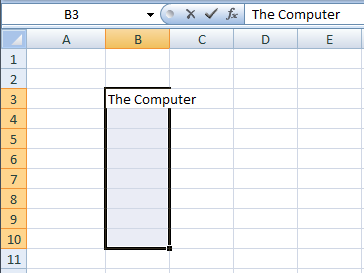
\includegraphics[scale=0.4]{src/images/chapter1_fig50.png}\qquad
\includegraphics[scale=0.4]{src/images/chapter1_fig51.png}
\end{figure}									

\section{सेल, रो और कॉलम को कॉपी एवं पेस्ट करना}\label{id-1.33}

जब आप सेल को स्थानांतरित (मूव) या कॉपी करते हैं, तो एक्सेल फॉर्मूलों एवं उनके परिणामी मानों, टिप्पणियों, सेल फॉर्मेट और हिडन सेलो, सहित पूरे सेल डेटा को मूव या कॉपी करता है। आप सेलों से विशिष्ट सामग्री (स्पेसिफिक कंटेंट्स) या विशेषताओं (ऐट्रिब्यूट्स) को भी कॉपी कर सकते हैं। आप बिना फार्मूला कॉपी किये उसके परिणामी मान को कॉपी कर सकते हैं, या आप केवल फार्मूला कॉपी कर सकते हैं। एक या एक से अधिक चयनित सेल, रो और कॉलम की कॉपी या मूव करने के लिए, आप \textbf{कट} कमांड या \textbf{कॉपी} कमांड या \textbf{माउस} का उपयोग कर सकते हैं। \textbf{कट} कमांड या \textbf{कॉपी} कमांड निम्न प्रकार से इस्तेमाल कि जा सकती हैंः

\begin{descriptionSimple}{चरण 1:}
\item[चरण 1]  एक या एक से अधिक सेल, रो और कॉलम जिसे आप कॉपी या मूव करना चाहते हैं उनका चयन करें
\item[चरण 2]  होम टैब पर, क्लिपबोर्ड ग्रुप में, निम्न में से एक करें:
		\begin{itemize}
		\item उन्हें मूव करने के लिए, कट क्लिक करें या कुंजीपटल शॉर्टकट  {\rm Ctrl + X}  का उपयोग करें	
		\item उन्हें कॉपी करने के लिए, कॉपी क्लिक करें या कुंजीपटल शॉर्टकट  {\rm Ctrl + C}  उपयोग करें
		\end{itemize}	
\item[चरण 3] एक रो या कॉलम के नीचे या दॅाये, राइट-क्लिक करें, जहाँ आप अपने चयन को मूव या कॉपी करना चाहते हैं और उसके बाद निम्न में से एक करें:
		\begin{itemize}
		\item जब आप उन्हें मूव कर रहे हैं, तब इन्सर्ट कट सेल क्लिक करें
		\item जब आप उन्हें कॉपी कर रहे हैं, तब इन्सर्ट कॉपी सेल क्लिक करें
		\end{itemize}
\end{descriptionSimple}

माउस का उपयोग करके आप एक या एक से अधिक सेल, रो और कॉलम को कॉपी या मूव निम्न प्रकार कर सकते हैं:

\begin{descriptionSimple}{चरण 1:}
\item[चरण 1]  एक या एक से अधिक सेल, रो और कॉलम जिसे आप कॉपी या मूव करना चाहते हैं का चयन करें
\item[चरण 2]  निम्न में से कोई एक कार्य करें:
		\begin{itemize}
		\item उन्हे मूव करने के लिए, चयन के बॉर्डर पर जाएँ, जब प्वाइंटर परिवर्तित होकर मूव प्वाइंटर बन जाए तब उनको किसी अन्य स्थान पर ड्रैग करें
		\item उन्हे कॉपी करने के लिए, चयन के बॉर्डर पर माउस प्वाइंटर को ले जाकर  {\rm Ctrl}  दबाएँ, जब प्वाइंटर परिवर्तित होकर कॉपी प्वाइंटर बन जाए तब उनको किसी अन्य स्थान पर ड्रैग करें
		\end{itemize}
\end{descriptionSimple}

सेलोें से विशिष्ट सामग्री (स्पेसिफिक कंटेंट्स) या विशेषताओं (ऐट्रिब्यूट्स) की कॉपी करने के लिए, जब आप सेलों को पेस्ट करे तब पेस्ट के नीचे तीर क्लिक करें, और निम्न रूप से विशिष्ट विकल्पो का चयन करें:

\begin{itemize}[topsep=-1ex,parsep=0ex,partopsep=0ex,itemsep=0.5ex]
\item केवल मानों को पेस्ट करने के लिए, \textbf{पेस्ट वैल्यू} पर क्लिक करें
\item केवल सेल के फॉर्मेट को पेस्ट करने के लिए, \textbf{पेस्ट स्पेशल} पर क्लिक करें और उसके बाद \textbf{पेस्ट} के अंतर्गत \textbf{फॉर्मेटस्} पर क्लिक करें
\item केवल फॉर्मूला पेस्ट करने के लिए, \textbf{फॉर्मूलास} पर क्लिक करें
\end{itemize}	
	
\section{सेलों को डेटा की एक श्रृंखला के साथ भरना}\label{id-1.34}

एक्सेल किसी वर्कशीट में कई सेलों में जानकारी को दोहराने के लिए कई तरीके प्रदान करता है। सन्निकट सेलों में जानकारी को दोहराने के लिए, फिल हैंडल का उपयोग करना सबसे सुविधाजनक तरीका है। यदि पहले सेल में कोई फार्मूला है, तो अतिरिक्त सेलो में फार्मूला दोहरा दिए जाएगा। और यदि पहले सेल में टेक्स्ट है, तो अतिरिक्त सेलों में टेक्स्ट दोहराया जाएगा। एक्सेल दिनांकों, महीनों, और अन्य स्थापित गैर-संख्यात्मक डेटा के पैटर्न को स्वतः भर (आटोफिल) देता हैं। यदि आपके द्वारा दर्ज जानकारी में एक्सेल एक पैटर्न (प्रतिमान) पहचानता है, तो अतिरिक्त सेलो में पैटर्न के अगले आइटम दर्ज हो जाएगें। उदाहरण के लिए, यदि पहले सेल में दिन रविवार है, एक्सेल सोमवार, मंगलवार, आदि के साथ निम्न सेल भर देगा।


फिल हैंडल का उपयोग करने के लिए, इच्छित सेलों का चयन करें, जिन्हे आप एक आधार के रूप में उपयोग करके अतिरिक्त सेलों को भरना चाहते हैं और फिर उन सेलों के पार (एक्रास) या नीचे फिल हैंडल को खींचे जिन्हे आप भरना चाहते हैं। आपके फिल हैंडल खींचने के बाद, आटो फिल विकल्प बटन प्रकट होता है, जिससे आप चयन का भरण कैसे होगा, के लिये विकल्पो को चुन सके। उदाहरण के लिए, केवल सेल स्वरूपों को भरने के लिए आप फिल फार्मेटिंग ओन्ली क्लिक करके चुन सकते हैं, या आप केवल सेल की सामग्री को भरने के लिए फिल विदाउट फार्मेटिंग क्लिक करके चुन सकते हैं।
				
\begin{figure}[t]
\centering
\includegraphics[scale=0.4]{src/images/chapter1_fig52.png}\quad
\includegraphics[scale=0.4]{src/images/chapter1_fig53.png}\quad
\includegraphics[scale=0.4]{src/images/chapter1_fig54.png}
\end{figure}

\section{सेल डेटा को संपादित करना}\label{id-1.35}

अपने एक्सेल वर्कशीट डेटा का संपादन (एडिट) करना बहुत आसान है। आप किसी भी निम्न तरीकों से अपने डेटा को संपादित कर सकते हैंः

\begin{itemize}[topsep=-1ex,parsep=0ex,partopsep=0ex,itemsep=0.5ex]
\item सेल का चयन करें जिसके डेटा को संपादित किया जाना हैं, और  {\rm F2}  दबाये, फिर   {\rm Backspace}  कुंजी का चयन करके गलत प्रविष्टि मिटाएँ (सही प्रविष्टि पुनः टाइप करें)
\item सेल का चयन करें और बस सही प्रविष्टि को पुनः लिखें
\item यदि आप केवल सेल की सामग्री को हटाना चाहते हैं, तो सेल का चयन करें और \textbf{डिलीट} कुंजी दबाएँ
\item पिछले प्रविष्टि वापस लाने के लिए, या तो स्टैण्डर्ड टूलबार पर \textbf{अनडु} बटन पर क्लिक करें या कुंजीपटल शॉर्टकट  {\rm Ctrl + Z}   का उपयोग करें
\end{itemize}

\section{फाइंड एंड रिप्लेस}\label{id-1.36}

एक्सेल की फाइंड (ढूँढना) एंड रिप्लेस (बदलना) सुविधा, एक बहुत शक्तिशाली टूल (उपकरण) है जो कि आपको तेजी से अपने वर्कशीट की सामग्री को बदलने देता है। किसी वर्कशीट में टेक्स्ट या मानों की स्थिति जानने, और (वैकल्पिक) प्रतिस्थापित करने के लिए फाइंड एंड रिप्लेस का उपयोग करें। स्वरूपण (फॉर्मेटिंग) को निर्दिष्ट (स्पेसिफ्यिंग) करके और साथ ही, केस मिलान (मैच केस) सहित अन्य खोज विकल्पो से, आप खोज परिणामों को संकुचित कर सकते हैं। किसी वर्कशीट मे टेक्स्ट और संख्याएँ, फाइंड एंड रिप्लेस करने के लिये निम्नलिखित चरणों का उपयोग करेःं

\begin{descriptionSimple}{चरण 1:}
\item[चरण 1] वर्कशीट में, किसी भी सेल पर क्लिक करें
\item[चरण 2] \textbf{होम} टैब पर, \textbf{एडिटिंग} ग्रुप मे, \textbf{फांइड \& सेलेक्ट} क्लिक करें
\item[चरण 3] निम्न करें:
		\begin{itemize}	
		\item टेक्स्ट या संख्याएँ ढूँढने के लिए, \textbf{फांइड} क्लिक करें
		\item टेक्स्ट या संख्याओ को ढूँढ कर बदलने के लिए, \textbf{रिप्लेस} क्लिक करें
		\end{itemize}
\item[चरण 4] \textbf{फांइड व्हाट} बॉक्स में, टेक्स्ट या संख्याएँ जिनको आप खोजना चाहते हैं को टाइप करें
\item[चरण 5] अपनी खोज को ओर आगे निर्धारित करने के लिये, \textbf{ऑप्शन्स} क्लिक करें और फिर निम्न में से कोई एक कार्य करें:
		\begin{itemize}	
		\item किसी वर्कशीट मे या संपूर्ण वर्कवुक मे, डेटा की खोज करने के लिए, \textbf{वीथिन} बॉक्स में, \textbf{शीट} या \textbf{वर्कबुक} का चयन करें
		\item विशिष्ट रो या कॉलमो में डेटा को खोजने के लिए, \textbf{सर्च} बॉक्स में, \textbf{बाई रो} या \textbf{बाई कॉलम} क्लिक करें
		\item विशिष्ट वर्णन के साथ डेटा को खोजने के लिए, \textbf{लुक-ईन} बॉक्स में, \textbf{फॉर्मुलास वैल्यूज} या \textbf{कमेेन्ट्स} क्लिक करें
		\item केस-संवेदी डेटा खोजने के लिए, मैच केस चेक बॉक्स का चयन करें	
		\item बस आपके द्वारा लिखे गए वर्णों वाले सेलो को खोजने के लिए \textbf{फाइंड व्हाट} बॉक्स में, \textbf{मैच ईंटायर सेल कंन्टेन्ट्स} चेक बॉक्स का चयन करें
		\end{itemize}
\end{descriptionSimple}					
\begin{figure}[H]
\centering
\includegraphics[scale=0.4]{src/images/chapter1_fig55.png}\qquad
\includegraphics[scale=0.4]{src/images/chapter1_fig56.png}
\end{figure}
\begin{figure}[H]
\centering
\includegraphics[scale=0.4]{src/images/chapter1_fig57.png}\qquad
\includegraphics[scale=0.4]{src/images/chapter1_fig58.png}
\end{figure}

\section{गो-टू सेल डेटा}\label{id-1.37}

वर्कशीट मे किसी विशिष्ट सेल पर जाने के लिए, आप गो-टू कंमाड का उपयोग कर सकते हैं। रेंजो के बीच मे जाने के लिए भी गो-टू कंमाड उपयोगी है। गो-टू डायलाग बॉक्स को प्रदर्शित करने के लिए आप थ्5 का उपयोग कर सकते हैं। आप निम्नानुसार गो-टू कंमाड का उपयोग कर सकते हैःं

\begin{descriptionSimple}{चरण 1:}
\item[चरण 1] वर्कशीट में, किसी भी सेल पर क्लिक करें
\item[चरण 2] \textbf{होम} टैब पर, \textbf{एडिटिंग} ग्रुप में, \textbf{गो-टू....} क्लिक करें या  {\rm F5}  प्रेस करें (गो-टू डायलाग बॉक्स प्रकट होगा)
\item[चरण 3] गो-टू स्क्रॉल बॉक्स मे कोई रेंज के नाम का चयन करें, या रिफरेंस टेक्स्ट बॉक्स में सेल लोकेशन लिखें
\item[चरण 4] उन्नत विकल्पो पर जाने के लिए, \textbf{स्पेशल} क्लिक करें और उपयुक्त विकल्प का चयन करें
\item[चरण 5] ओके क्लिक करें
\end{descriptionSimple}
\begin{figure}[H]
\centering
\includegraphics[scale=0.45]{src/images/chapter1_fig59.png}\qquad
\includegraphics[scale=0.45]{src/images/chapter1_fig60.png}
\end{figure}				

\section{स्प्लिट पैन और फ्रीज पैन के द्वारा रो और कॉलम को लॉक करना}\label{id-1.38}

स्प्लिट पैन और फ्रीज पैन के माध्यम से आप एक वर्कशीट के अनुभागो को एक ही जगह स्थिर (होल्ड़) कर सकते हैं ताकी वे वर्कशीट मे स्क्रॉल करने के दौरान हमेशा दिखाई दे। यह बड़े वर्कशीटो के लिए विशेष रूप से उपयोगी है क्योंकि आप अपने डेटा मे स्क्रॉल करने के दौरान, कॉलम और रो शीर्षोंको को एक ही जगह स्थिर कर सकते हैं। यदि आपके स्प्रेडशीट की पहली रो हैडर्स रखती है तो आप उस रो को स्थिर (फ्रीज) करना चाहेंगे, यह सुनिश्चित करने के लिए कि स्प्रेडशीट में नीचे स्क्रॉल करने के दौरान कॉलम हैडर्स दृश्यमान रहें। रो या कॉलमो को स्थिर करने के लिए निम्न चरणों उपयोग करेः 

\begin{descriptionSimple}{चरण 1:}
\item[चरण 1] रो के नीचे उस रो के लेबल पर क्लिक करें, जिसे आप वर्कशीट के शीर्ष पर स्थिर करना चाहते हैं
\item[चरण 2] \textbf{व्यू} टैब के \textbf{विंडो} ग्रुप में \textbf{फ्रीज पैन} क्लिक करें
\item[चरण 3] निम्न में से एक करेंः
		\begin{itemize}
		\item केवल एक रो स्थिर करने के लिए, शीर्ष \textbf{फ्रीज टॉप रो} क्लिक करें
		\item केवल एक कॉलम स्थिर करने के लिए, \textbf{फ्रीज फस्ट कॉलम} पर क्लिक करें
		\item एक से अधिक रो या कॉलम स्थिर करने के लिए, या एक ही समय में दोनों रो और कॉलमो को स्थिर करने के लिए, \textbf{फ्रीज पैन} पर क्लिक करें (आपको अपने कर्सर को उन रो के नीचे और उन कॉलमो के दाईं करना होगा, जिन्हे आप स्थिर करना चाहते हैं)
		\item एक से अधिक रो को स्थिर करने के लिए (रो 1 के साथ शुरू), उस अंतिम रो जहॉ तक आप स्थिर करना चाहते है के नीचे की रो का चयन करें, \textbf{फ्रीज पैन} पर क्लिक करें
		\item एक से अधिक कॉलमो को स्थिर करने के लिए, उस अंतिम कॉलम जहॉ तक आप स्थिर करना चाहते है के दाईं ओर के कॉलम का चयन करें, \textbf{फ्रीज पैन} पर क्लिक करें
		\end{itemize}
\item[चरण 4] फ्रीज़् किए गए पैनस् को हटाने के लिए, \textbf{अन-फ्रीज पैन} क्लिक करें
\end{descriptionSimple}

आप वर्कशीट विंडो को अलग-अलग फलकों (पैनस्) में भी विभाजित कर सकते हैं और वर्कशीट को प्रत्येक फलक में स्क्रॉल कर सकते है, ताकि आप आसानी से दो अलग-अलग वर्कशीट स्थानो केे डेटा की तुलना कर सके। स्प्लिटिंग पैन आपको वर्कशीट के कई एरियों को एक ही बार में देखने की सुविधा देता है। किसी वर्कशीट को फलको में विभाजित करने के लिए निम्न चरणों का पालन करेःं

\begin{descriptionSimple}{चरण 1:}
\item[चरण 1] सेल का चयन करें, जहाँ से आप वर्कशीट को विभाजित करना चाहते हैं (वर्कशीट सक्रिय सेल के ऊपर और बाईं ओर से विभाजित हो जाएगा और चार फलक बनगें)
\item[चरण 2] \textbf{विंडो} ग्रुप  में, \textbf{व्यू} टैब के, \textbf{स्प्लिट} बटन पर क्लिक करें
\end{descriptionSimple}

वर्कशीट अनुभागो (सेक्सन) में विभाजित हो जायेगी, जिनमे से प्रत्येक अनुभाग को अन्य अनुभागो को मूव किये बिना नेविगेट किया जा सकता हैं। आप विभाजन के स्थान को, पैन पर क्लिक कर और उसे खींचकर, भी समायोजित कर सकते हैं। फिर से विभाजन को हटाने के लिए स्पिलिट बटन क्लिक करें।

\begin{figure}[H]
\centering
\includegraphics[scale=0.6]{src/images/chapter1_fig61.png}\\[4pt]
\includegraphics[scale=0.6]{src/images/chapter1_fig62.png}
\end{figure}
\begin{figure}[H]
\centering
\includegraphics[scale=0.6]{src/images/chapter1_fig63.png}
\end{figure}

\section{वर्तनी जाँच करना}\label{id-1.39}

एक्सेल मे एक अंतर्निहित वर्तनी (स्पेलिंग) परीक्षक (चेकर) होता हैं, जिससे आप अपनी वर्कशीट में वर्तनी की त्रुटियो और लेखन त्रुटियो को ढूॅंढकर उन्हे दुर कर सकते है। यदि आपकी वर्कबुक मे एक से अधिक शीटे है तब आप वर्तनी परीक्षक को प्रारंभ करने से पहले इच्छित शीटों का चयन कर सकते हैं जिनकी आपको जॉच करनी हैं। पहले उन सम्बधित सेलो का चयन करके आप बस प्रविष्टियों के एक विशेष ग्रुप की वर्तनी जाँच भी कर सकते हैं। किसी वर्कशीट में वर्तनी की जाँच करने के लिए, निम्न चरणों का पालन करेंः

\begin{descriptionSimple}{चरण 1:}
\item[चरण 1] \textbf{रिव्यु} टैब के, \textbf{प्रूफिंग} ग्रुप में, \textbf{स्पेलिंग} पर क्लिक करें (या  {\rm F7}  दबाएँ)\\  (एक्सेल, वर्कशीट में टेक्स्ट प्रविष्टियों की वर्तनी की जाँच शुरू कर देेता है। जब वर्तनी परीक्षक, किसी अज्ञात शब्द को देखता है, यह स्पेलिंग डायलाग बॉक्स मे प्रदर्शित करता है। एक्सेल \textbf{नॉट इन डिक्शनरी} टेक्स्ट बॉक्स में दिखाए गए अज्ञात शब्द के लिए, सजेशन लिस्ट बॉक्स मे संभावित प्रतिस्थापन (रिप्लेसमेंट) बताकर, उपलब्ध प्रतिस्थापनो का सुझाव देता हैं। यदि प्रतिस्थापन गलत है, तब आप सजेशन लिस्ट मे स्क्रॉल करके सही प्रतिस्थापन पर क्लिक कर सकते हैं)
\item[चरण 2] एक या एक से अधिक निम्न डायलाग बॉक्स विकल्पों में से चयन करेंः
		\begin{itemize}
		\item \textbf{इग्नोर वन्स} या \textbf{इग्नोर आल:}जब एक्सेल का वर्तनी परीक्षक एक ऐसे शब्द को देखता है जो उसके शब्दकोश के अनुसार संदिग्ध है, लेकिन आपको पता है कि वह शब्द व्यवहार्य (वाइबल) है, तब इग्नोर वन्स बटन क्लिक करें। यदि आप नहीं चाहते, कि वर्तनी परीक्षक इस शब्द के बारे में आगे फिर से क्वेरी करे, तब इग्नोर आल क्लिक करें
		\item \textbf{ऐड टू डिक्शनरी:}अज्ञात शब्द को कस्टम शब्दकोश में जोड़ने के लिए इस बटन पर क्लिक करें ताकि एक्सेल इसे फिर से फ्लैग (चिह्नक) नहीं करें
		\item \textbf{चेंज:}टेक्स्ट बॉक्स \textbf{नॉट इन डिक्शनरी} में सूचीबद्ध शब्द को, सजेशन लिस्ट बॉक्स मे चयनित शब्द से प्रतिस्थापित करने के लिए इस बटन पर क्लिक करें
		\item \textbf{चेंज आल:}वर्कशीट में इस अशुद्ध वर्तनी वाले शब्द की सभी आवृत्तियों को बदलने के लिए, सजेशन लिस्ट बॉक्स मे चयनित शब्द से प्रतिस्थापित करने के लिए इस बटन पर क्लिक करें
		\item \textbf{ऑटोकोर्रेक्ट:}एक्सेल द्वारा स्वचालित रूप से सजेशन लिस्ट बॉक्स मे चयनित सुझाव के साथ इस वर्तनी त्रुटि को ठीक करने के लिए इस बटन पर क्लिक करें (ऑटोकोर्रेक्ट डायलाग बॉक्स में वर्तनी त्रुटि और सुझाव को जोड़कर)
		\end{itemize}
\item[चरण 3] वर्तनी जाँच पूर्ण होने पर ओके क्लिक करें
\end{descriptionSimple}
\begin{figure}[H]
\centering
\includegraphics[scale=0.6]{src/images/chapter1_fig64.png}
\end{figure}
					
\section{ऑटोकोरेक्ट}\label{id-1.40}

लेखन त्रुटियों, कैपिटलाइजेशन त्रुटियों और गलत वर्तनी वाले शब्दों को सही करने, साथ ही प्रतीकों और टेक्स्ट के अन्य भागो को स्वचालित रूप से सम्मिलित करने के लिए आप ऑटोकोरेक्ट  (स्वतः सुधार) सुविधा का उपयोग कर सकते हैं। डिफॉल्ट रूप से, ऑटोकोरेक्ट आमतौर पर गलत वर्तनियों और प्रतीकों की एक मानक सूची का उपयोग करता है, लेकिन आप इस सूची में प्रविष्टियों को संशोधित भी कर सकते हैं। इस सूची में प्रविष्टियों को संशोधित करने के लिए आप निम्न चरणों का उपयोग करके ऑटोकोरेक्ट डायलाग बॉक्स खोल सकते हैंः

\begin{descriptionSimple}{चरण 1:}
\item[चरण 1] \textbf{ऑफिस} बटन क्लिक करें और फिर \textbf{एक्सेल ऑप्शन्स} क्लिक करें
\item[चरण 2] \textbf{प्रूफिंग} क्लिक करें, और \textbf{ऑटोकोरेक्ट ऑप्शन्स} क्लिक करें
\item[चरण 3] आवश्यकता अनुसार प्रविष्टियो को संशोधित करें
\end{descriptionSimple}
\begin{figure}[H]
\centering
\includegraphics[scale=0.3]{src/images/chapter1_fig65.png}\qquad
\includegraphics[scale=0.3]{src/images/chapter1_fig66.png}
\end{figure}
\begin{figure}[H]
\centering
\includegraphics[scale=0.4]{src/images/chapter1_fig67.png}
\end{figure}												

\section{ट्रैक चेंजेंस}\label{id-1.41}

हर बार जब आप किसी वर्कबुक को सहेजें, वर्कबुक परिवर्तनों के बारे में विवरण को अभिलेख (लॉग) करने के लिए ट्रैक चेंजेंस का उपयोग कर सकते हैं। यह परिवर्तन इतिहास, डेटा वर्कबुक में किए गए किसी भी परिवर्तन की पहचान करने मे मदद कर सकते हैं, और उसके बाद आप उन परिवर्तनों को स्वीकार या अस्वीकार कर सकते हैं। चेंज ट्रैकिंग विशेष रूप से उपयोगी होता है जब कई उपयोगकर्ता एक वर्कबुक संपादित करें। जब आप किसी वर्कबुक को टिप्पणियों के लिए समीक्षकों को सबमिट करें, और उसके बाद प्राप्त इनपुट को उस वर्कबुक की एक कॉपी में मर्ज करने, चेंज और टिप्पणियाँ जिसे आप रखना चाहते है, उनको शामिल करने के लिए भीे यह उपयोगी है।


जब आप ट्रैक चेंजेंस सुविधा को शुरु कर देते है उसके बाद आपके द्वारा संपादित हर सेल एक अद्वितीय सीमा (यूनिक बॉर्डर) और संकेतक (इंडिकेटर) के द्वारा विशिष्ट रूप से दर्शाता (हाइलाइट) हैं। एक चिह्नित सेल का चयन परिवर्तनो का विवरण दिखाएगा। यह आपको और अन्य समीक्षको को किसी संशोधन को स्थायी रूप से स्वीकार करने से पहले, क्या बदल दिया गया है यह देखने के लिए अनुमति देता है। एक वर्कबुक मे ट्रैक चेंजेंस चालू करने के लिए निम्न चरणों का पालन करेंः
				
\begin{descriptionSimple}{चरण 1:}
\item[चरण 1] \textbf{रिव्यु} टैब केे, \textbf{चेंजेस} ग्रुप मे, \textbf{शेयर वर्कबुक} क्लिक करें
\item[चरण 2] \textbf{एडिटिंग} टैब पर, \textbf{अलाऊ चेंजेस बाई मोर दैन वन यूजर एट द सेम टाइम} चेक बॉक्स का चयन करें
\item[चरण 3] \textbf{एडवांस्ड} टैब क्लिक करें
\item[चरण 4] \textbf{ट्रैक चेंजेस} के तहत, \textbf{कीप चेंज हिस्ट्री फॉर} क्लिक करें और, \textbf{डेज} बॉक्स में, इच्छित दिनों जितनो का परिवर्तन इतिहास आप रखना चाहते है, उनकी संख्या को लिखे
\item[चरण 5] ओके क्लिक करें, और फिर वर्कबुक को सहेजने के लिए ओके क्लिक करें
\end{descriptionSimple}
\begin{figure}[H]
\centering
\includegraphics[scale=0.4]{src/images/chapter1_fig68.png}\qquad
\includegraphics[scale=0.4]{src/images/chapter1_fig69.png}
\end{figure}
\begin{figure}[H]
\centering
\includegraphics[scale=0.4]{src/images/chapter1_fig70.png}
\end{figure}				
					
\section{परिवर्तनो को स्वीकारना और अस्वीकारना}\label{id-1.42}

परिवर्तनो को, स्वीकार और अस्वीकार करने के लिए निम्न चरणों का पालन करेःं

\begin{descriptionSimple}{चरण 1:}
\item[चरण 1] \textbf{रिव्यु} टैब के, \textbf{चेंजेस} ग्रुप मे, \textbf{ट्रैक चेंजेस} को क्लिक करें, और फिर \textbf{एक्सेप्ट ओर रिजेक्ट चेंजेस} क्लिक करें
\item[चरण 2] यदि वर्कबुक सहेजने के लिए कहॉ जाये तब ओके क्लिक करें
\item[चरण 3] \textbf{सेलेक्ट चेंजेस टू एक्सेप्ट ओर रिजेक्ट} डायलाग बॉक्स में, उपयुक्त विकल्प चुनें
\item[चरण 4] ओके क्लिक करें, और फिर \textbf{एक्सेप्ट ओर रिजेक्ट चेंजेस} डायलाग बॉक्स में प्रत्येक परिवर्तन के बारे में जानकारी की समीक्षा करें
\item[चरण 5] प्रत्येक परिवर्तन को स्वीकार या अस्वीकार करने के लिए, \textbf{एक्सेप्ट} या \textbf{रिजेक्ट} क्लिक करें
\item[चरण 6] एक सेल के लिए मान का चयन करने के लिए कहा जाये तो इच्छित मान क्लिक करें, और उसके बाद \textbf{एक्सेप्ट} क्लिक करें
\end{descriptionSimple}
\begin{figure}[H]
\centering
\includegraphics[scale=0.5]{src/images/chapter1_fig71.png}
\end{figure}
\begin{figure}[H]
\centering
\includegraphics[scale=0.5]{src/images/chapter1_fig72.png}
\end{figure}								

\section{कमेंटस्}\label{id-1.43}

कभी-कभी आप किसी सेल की सामग्री संपादित करने के बजाय, प्रतिक्रिया प्रदान करने के लिए एक टिप्पणी (कमेंट) जोड़ना चाह सकते हैं। कमेंटस् का उपयोग कर, आप कोई वर्कशीट डेटा के लिए अतिरिक्त प्रसंग प्रदान करके, उसे समझना आसान बना सकते हैं। उदाहरण के लिए, आप एक अलग-अलग सेल में डेटा के बारे में जानकारी प्रदान करने के लिये, एक नोट के रूप में एक कमेंट का उपयोग कर सकते हैं। आप डेटा जिसे एक उपयोगकर्ता को दर्ज करना चाहिए, पर मार्गदर्शन प्रदान करने के लिए, एक कॉलम शीर्ष पर भी एक कमेंट जोड़ सकते हैं। जब किसी सेल मे कमेंट होता है, तब एक लाल संकेतक सेल के कोने में दिखाई देता है। जब आप सेल पर सूचक को ले जायेंगे तब कमेंट दिखाई देता है। एक सेल मे एक कमेंट जोड़ने के लिए निम्न चरणों का पालन करेःं

\begin{descriptionSimple}{चरण 1:}
\item[चरण 1] उस सेल का चयन करें जहॉ आप एक कमेंट जोड़ना चाहते हैं
\item[चरण 2] \textbf{रिव्यु} टैब के, \textbf{कमेंट} ग्रुप  में, \textbf{न्यू कमेंट} क्लिक करें
\item[चरण 3] कमेंट के मुख्य भाग में, कमेंट टेक्स्ट लिखें
\item[चरण 4] कमेंट बॉक्स के बाहर क्लिक करें, कमेंट बॉक्स गायब हो जाता है, लेकिन कमेंट को दृ श्यमान रखने के लिए कमेंट संकेत बना रहता है, निम्न कार्य करेंः
		\begin{itemize}
		\item सेल का चयन करें
		\item \textbf{रिव्यु} टैब केे, \textbf{कमेंट} ग्रुप में, \textbf{शो/हाईड कमेंट} क्लिक करें (आप कमेंट वाले सेल पर राइट-क्लिक करके भी, और फिर शो/हाईड कमेंट पर क्लिक कर सकते हैं)
		\end{itemize}
\end{descriptionSimple}
\medskip

\begin{figure}[H]
\centering
\includegraphics[scale=0.6]{src/images/chapter1_fig73.png}
\end{figure}				

\section*{महत्वपूर्ण बिंदुः}

\begin{itemize}[topsep=-1ex,parsep=0ex,partopsep=0ex,itemsep=0.5ex]
\item एक्सेल एक स्प्रेडशीट एप्लीकेशन हैं, जिसे माइक्रोसॉफ्ट द्वारा विकसित किया गया हैं।
\item एक स्प्रेडशीट मूलतः रो और कॉलमो की एक मैट्रिक्स होती हैं।
\item एक्सेल प्राथमिक रूप से संख्यात्मक परिकलन के लिए है, जबकि वर्ड एक शब्द संसाधक (प्रोसेसर) होता हैं।
\item एक्सेल का प्राथमिक उद्देश्य बुनियादी और जटिल गणितीय परिकलन करना हैं।
\item एक एक्सेल फाइल एक वर्कबुक होती हैं, जिसमे एक या एक से अधिक वर्कशीटे हो सकती हैं।
\item एक एक्सेल वर्कशीट एकल (सिंगल) स्प्रेडशीट हैं, जो रो (संख्याओं द्वारा निर्दिष्ट) और कॉलमों (अक्षरों द्वारा निर्दिष्ट) की मैट्रिक्स होती है।
\item सॉर्ट (क्रमवार लगाना) एक सामान्य स्प्रेडशीट कार्य हैं जिससे आप आसानी से अपने डेटा को पुनः व्यवस्थित कर सकते हैं।
\item आप डेटा को फिल्टर (अलग करना) करके केवल उन्ही रो को प्रदर्शित कर सकते हैं जो आपके द्धारा निर्दिष्ट किये गये मापदंड से मेल खाती हैं, और उन रो को छुपा सकते हैं जिन्हे आप प्रदर्शित नहीं करना चाहते हैं।
\item हैडर जानकारी का वो भाग हैं, जो दस्तावेज के मुख्य भाग के ऊपर प्रिंट किया जाता है और फूटर जानकारी का वो भाग हैं, जो दस्तावेज के मुख्य भाग के नीचे प्रिंट किया जाता हैं।
\item आप प्रिंट डायलाग बॉक्स के, प्रिंट रेंज अनुभाग में, उपयुक्त विकल्पो का उपयोग करके पेजों की एक श्रेणी को प्रिंट कर सकते हैं।
\item आप तीन प्रकार का डेटा एक्सेल में दर्ज करते हैंः टेक्स्ट, मान (संख्या), या सूत्र (फार्मूला)।
\item एक्सेल दिनांकों, महीनों, और अन्य स्थापित गैर-संख्यात्मक डेटा के पैटर्न को स्वतः भर (आटोफिल) देता हैं।
\item एक्सेल की फाइंड एंड रिप्लेस सुविधा, एक बहुत शक्तिशाली टूल (उपकरण) है जो कि आपको तेजी से अपने वर्कशीट की सामग्री को बदलने देता है।
\item किसी वर्कशीट में टेक्स्ट या मानों की स्थिति जानने, और (वैकल्पिक) प्रतिस्थापित करने के लिए फाइंड एंड रिप्लेस का उपयोग करें।
\item वर्कशीट मे किसी विशिष्ट सेल पर जाने के लिए, आप गो-टू कंमाड का उपयोग कर सकते हैं।
\item स्प्लिट पैन और फ्रीज पैन के माध्यम से आप एक वर्कशीट के अनुभागो को एक ही जगह स्थिर (होल्ड़) कर सकते हैं ताकि वे वर्कशीट मे स्क्रॉल करने के दौरान हमेशा दिखाई दे।
\end{itemize}

\section*{अभ्यासार्थ प्रश्न}

\def\paragraphTitle#1{\medbreak\noindent{\bfseries #1}}
\paragraphTitle{वस्तुनिष्ठ प्रश्नः}
\begin{descriptionSimple}{प्रश्न 1.}
\item[\textbf{प्रश्न 1}] एक सुविधा (फीचर) है, जो केवल निर्दिष्ट मापदंड के अनुसार डेटा को कॉलम में प्रदर्शित करता है

	\begin{tabular}{llll}
	\textbf{अ.}  फार्मूला & \textbf{ब.}  सार्टिंग & \textbf{स.}  फिल्टरिंग & \textbf{द.} पाइवोट (च्पअवज)
	\end{tabular}

\item[\textbf{प्रश्न 2}] किसी कॉलम के आइटम्स को कुछ अनुक्रम या क्रम (सीक्वेंस या आर्डर) में व्यवस्थित करने की प्रक्रिया को कहा जाता हैः

	\begin{tabular}{llll}
		\textbf{अ.}  अरेजिंग & 
		\textbf{ब.} ऑटोफिल & 
		\textbf{स.} सार्टिंग &
		\textbf{द.} फिल्टरिंग
	\end{tabular}		
\item[\textbf{प्रश्न 3}] जब हम एक नया एक्सेल फाइल बनाते हैं, तब उसमें डिफॉल्ट रूप से कितने शीट होते हैं?

		\begin{tabular}{llll}
		\textbf{अ.}  1  &
		\textbf{ब.} 3  &
		\textbf{स.} 5  &
		\textbf{द.} 10
		\end{tabular}
\item[\textbf{प्रश्न 4}] कंडीशनल फोर्मेटिंग (सशर्त स्वरूपण) के बारे में, निम्नलिखित में से कौन सच नहीं है?

		\begin{tabular}{p{.9\textwidth}}
		\textbf{अ.}  जाँच करने के लिए आप एक से अधिक कंडीशन (शर्त) जोड़ सकते हैं\\
		\textbf{ब.} बोल्ड देखने के लिए आप कंडीशन सेट कर सकते हैं और इटैलिक को उन पर लागू सकते हैं \\
		\textbf{स.} जो निर्दिष्ट शर्तों को पूरा करता है आप उन पर फॉन्ट, बॉर्डर और पैटर्न फॉर्मेट लागू कर सकते हैं\\
		\textbf{द.} कंडीशनल फोर्मेटिंग डायलाग बॉक्स से आप किसी भी कंडीशन को हटा सकते हैं, जो आवश्यक नहीं है
		\end{tabular}
\item[\textbf{प्रश्न 5}] निम्न में से किसका उपयोग करके, एक सेल फॉर्मेट को किसी अन्य सेल पर कॉपी किया जा सकता हैं ?

		\begin{tabular}{llll}
		\textbf{अ.}  फॉर्मेट पेंटर & 
		\textbf{ब.} फॉर्मेट सेटिंग &
		\textbf{स.} फॉर्मेट शोविंग &
		\textbf{द.} फॉर्मेट चेकिंग 
		\end{tabular}
\item[\textbf{प्रश्न 6.}] सभी फार्मूलो को किस प्रतीक (सिंबल) के साथ शुरू करना चाहिए?

		\begin{tabular}{llll}
		\textbf{अ.}  =  & 
		\textbf{ब.}  +  &
		\textbf{स.} (  &
		\textbf{द.} @ 
		\end{tabular}
\item[\textbf{प्रश्न 7}] जो कुंजी आप वर्तनी (स्पेलिंग) की जाँच करने के लिए दबाते है?

		\begin{tabular}{llll}
		\textbf{अ.}  F3 &
		\textbf{ब.} F5 &
		\textbf{स.} F7 &
		\textbf{द.} F9
		\end{tabular}
\end{descriptionSimple}

\paragraphTitle{अतिलघूत्तरात्मक प्रश्नः}
\begin{descriptionSimple}{\textbf{प्रश्न 1.}}
\item[\textbf{प्रश्न 1}] क्या एमएस वर्ड में उन्नत स्वरूपण सुविधाऐं (एडवांस्ड फोर्मेटिंग फैसिलिटीज) होती है?
\item[\textbf{प्रश्न 2}] डिफॉल्ट रूप से, एक्सेल किसी वर्कबुक में कितनी वर्कशीट प्रदान करता हैं?
\item[\textbf{प्रश्न 3}] किस कंमाड का उपयोग वर्कबुक को सहेजने के लिए किया जाता है?
\item[\textbf{प्रश्न 4}] नेविगेशन बटन एक्सेल वर्कबुक में ....... के कोने मे प्रस्तुत होते हैं।
\item[\textbf{प्रश्न 5}] हैडर्स और फूटर्स केवल ........... व्यू और प्रिंट पेजों में प्रदर्शित हैं।
\item[\textbf{प्रश्न 6}] एक्सेल मे, टेक्स्ट और मान प्रविष्टियाँ सेल मे किस ओर संरेखित (एलाइन) होती हैं?
\item[\textbf{प्रश्न 7}] गो-टू डायलाग बॉक्स को प्रदर्शित करने के लिए किस कंमाड का उपयोग किया जाता है?
\item[\textbf{प्रश्न 8}] कौन-सा बटन वर्कशीट में टेक्स्ट प्रविष्टियों की वर्तनी (स्पेलिंग) की जाँच करने के लिए उपयोग किया जाता है?
\item[\textbf{प्रश्न 9}] एक्सेल में आप रो/कॉलम को क्यो हाइड (छुपाना) करते हैं?
\end{descriptionSimple}

\paragraphTitle{लघूत्तरात्मक प्रश्नः}
\begin{descriptionSimple}{\textbf{प्रश्न 1.}}
\item[\textbf{प्रश्न 1}] माइक्रोसॉफ्ट एक्सेल क्या होता है?
\item[\textbf{प्रश्न 2}] एमएस वर्ड की एमएस एक्सेल के साथ तुलना करें।
\item[\textbf{प्रश्न 3}] वर्कवुक और वर्कशीट को परिभाषित करंे।
\item[\textbf{प्रश्न 4}] एक्सेल में लेबलिंग से आपका क्या समझते हैं?
\item[\textbf{प्रश्न 5}] एक्सेल में आप एक नई शीट कैसे जोड़ सकते हैं ?
\item[\textbf{प्रश्न 6}] एमएस एक्सेल में नेविगेशन कुंजियाँ (कीज्) क्या होती हैं?
\item[\textbf{प्रश्न 7}] एक्सेल में मर्ज और स्पिलिट को समझाएँ।
\item[\textbf{प्रश्न 8}] एक्सेल में हैडर्स और फूटर्स बनाने के लिए चरणों को समझाएँ।
\item[\textbf{प्रश्न 9}] सॉर्टिंग से आप क्या समझते हैं? एक्सेल में सॉर्ट करने के लिए चरणों को समझाएँ।
\item[\textbf{प्रश्न 10}] एक्सेल में फार्मूला को उपयोग करने के क्या लाभ है?
\item[\textbf{प्रश्न 11}] हैडर्स और फूटर्स पर संक्षिप्त टिप्पणी लिखे।
\item[\textbf{प्रश्न 12}] गो-टू कंमाड क्या है?					
\end{descriptionSimple}					
\newpage

\paragraphTitle{निबंधात्मक प्रश्नः}
\begin{descriptionSimple}{\textbf{प्रश्न 1.}}
\item[\textbf{प्रश्न 1}] एक्सेल में जानकारी प्रविष्ट करने को विस्तार मे समझाएँ।
\item[\textbf{प्रश्न 2}] ट्रैक चेजेंस क्या होते है? एक वर्कबुक के लिए चेंज ट्रैकिंग चालू करने के लिए चरणों को समझाएँ।
\item[\textbf{प्रश्न 3}] फाइंड और रिप्लेस सुविधा का क्या उपयोग है? फाइंड और रिप्लेस करने के लिए चरणों को समझाएँ।
\item[\textbf{प्रश्न 4}] वर्कशीट में सेल, रो और कॉलम को इन्सर्ट करने के लिए चरणों को समझाएँ।
\item[\textbf{प्रश्न 5}] आप हैडर्स और फूटर्स के लिए मार्जिन कैसे सेट कर सकते हैं?
\item[\textbf{प्रश्न 6}] फिल्टर और सॉर्ट आपरेशन को विस्तार मे समझाएँ।
\item[\textbf{प्रश्न 7}] एक्सेल में फंक्शन और फार्मूला के बीच मे क्या अंतर होता है?
\item[\textbf{प्रश्न 8}] स्प्लिट पैन्स और फ्रीजिंग पैन्स के द्वारा रो और कॉलम को लॉक करना समझाएँ।
\end{descriptionSimple}

\paragraphTitle{उत्तरमाला}

\begin{tabular}{@{}llll}
\textbf{उत्तर 1:} स & 
\textbf{उत्तर 4:} ब &
\textbf{उत्तर 2:} स &
\textbf{उत्तर 5:} अ\\
\textbf{उत्तर 3:} ब &
\textbf{उत्तर 6:} अ &
\textbf{उत्तर 7:} स	&		
\end{tabular}
